\documentclass[10pt]{IEEEtran}
\usepackage{etex}
\usepackage{epsfig}
\usepackage{amsmath}
\usepackage{multirow}
\usepackage{tabularx}
\usepackage{booktabs}
\usepackage{amsmath,graphicx}
\usepackage{pgf}
\usepackage{tikz}
\usepackage{subfig}
\usetikzlibrary{backgrounds,shapes,snakes}
\usetikzlibrary{calc,chains,positioning,patterns}
\usepackage{phaistos}
\usepackage{cases}
\usepackage{pgfplots}
\usepackage{cite}


\begin{document}

\newlength\figureheight
\newlength\figurewidth
\setlength\figureheight{2.3cm}
\setlength\figurewidth{0.35\textwidth}


\title{RETF-Independent Multi-Channel Late Reverberant Power Spectral Density Estimator}

\author{Ina Kodrasi,~\IEEEmembership{Member,~IEEE,}
        Simon Doclo,~\IEEEmembership{Senior Member,~IEEE}
\thanks{The authors are with the Signal Processing Group, Department of Medical Physics and Acoustics, and Cluster of Excellenece Hearing4All, University of Oldenburg, Germany (email: ina.kodrasi@uni-oldenburg.de, simon.doclo@uni-oldenburg.de).}% <-this % stops a space
\thanks{
This work was supported in part by the Cluster of Excellence 1077 ``Hearing4All'', funded by the German Research Foundation (DFG), the Marie Curie Initial Training Network DREAMS (Grant no. 316969), and the joint Lower Saxony-Israeli Project ATHENA, funded by the State of Lower Saxony.
}
\thanks{Manuscript received xx; revised xx.}}


\maketitle

\begin{abstract}
\end{abstract}

\begin{IEEEkeywords}
\end{IEEEkeywords}

\section{Introduction}

\IEEEPARstart{T}{his} 

\section{Configuration and Notation}
Consider a reverberant and noisy acoustic system with a single speech source and $M \geq 2$ microphones as depicted in Fig.~\ref{fig: ac_sys}.
The $m$-th microphone signal $Y_m(k,l)$ at frequency index $k$ and frame index $l$ is given by 
\begin{figure}[b!]
  \centering
  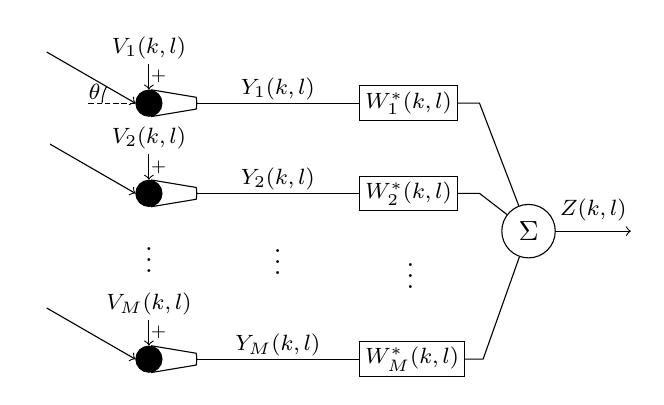
\begin{tikzpicture}
    % Adjustments
    \def\micd{.1cm}                % mic diameter
    \def\micl{.6cm}                % mic length
    \def\micw{.15cm}                % mic width
   \def\micbend{10}               % mic bottom bend
    \def\micdistance{.8cm}         % distance between microphones
    \def\filterdistance{2.5cm}     % distance between microphone and filter
    \def\filteroutline{.9cm}       % length of line which gets out of filter
    \def\sumdistance{1.5cm}        % distance of sum node to the filter
    \def\sumoutline{1cm}           % length of line which gets out of sum
    \def\headdistance{2cm}         % distance between microphone and head

    % Styles
    \tikzset{%
      mic head/.style={fill=black,draw=black,circle,minimum size=\micd},
      filter/.style={draw,minimum width=1.1cm,inner sep=2pt},
      sum/.style={draw,circle},
      xlabel/.style={inner sep=1pt,above,midway},
      sumlabel/.style={xlabel},
      hlabel/.style={xlabel,sloped,pos=.7},
      head/.style={font=\Large}
    }

    % Draw Microphones
    \begin{scope}[start chain=going below,every node/.style={on chain},node distance=\micdistance]
      \node[mic head] (mic1) {};
      \node[mic head] (mic2) {};
      \node[mic head,yshift=-1.2*\micdistance] (mic3) {};
    \end{scope}
    %\node[yshift=3pt] at ($(mic2)!.5!(mic3)$) {$\vdots$};

    \foreach \m in {1,2,3} {%
      \coordinate (m1) at ($(mic\m)+(\micl,\micw/2)$);
      \coordinate (m2) at ($(mic\m)+(\micl,-\micw/2)$);
      \draw (tangent cs:node=mic\m,point={(m1)},solution=1) -- (m1) to[bend left=\micbend] (m2) -- (tangent cs:node=mic\m,point={(m2)},solution=2);
    }

    % Draw Filter
    \foreach \m/\i in {1/1,2/2,3/M} {%
      \node[filter,right=\filterdistance of mic\m] (filter\m) {\footnotesize $W^{*}_{\i}(k,l)$};
      \draw ($(mic\m)+(\micl,0)$) to node[xlabel] (x\m) {\footnotesize $Y_{\i}(k,l)$} (filter\m);
    }
    \node[yshift=3pt] at ($(mic2)!.4!(mic3)$) {$\vdots$};
    \node[yshift=3pt] at ($(filter2)!.5!(filter3)$) {$\vdots$};
    \node[yshift=3pt] at ($(x2)!.5!(x3)$) {$\vdots$};
    % Sum Node
    \node[sum] (sum) at ($(filter1)!.5!(filter3)+(\sumdistance,0)$) {$\Sigma$};
    \draw[->] (sum) -- node[above] {\footnotesize $Z(k,l)$} ++(1.3,0);
    % Connect filter with sum
    \foreach \m in {1,2,3} {%
      \draw (filter\m) -- ++(\filteroutline,0) -- (sum);
    }

    % Connect head with mics
    \foreach \m/\i in {1/1,2/2,3/M} {%
      \draw[<-] (mic\m.west) -- ++(150:1.3cm) coordinate (c\m);
%      \draw[->] (head) --  (mic\m);
    }
    % Head
    \node[head,left] (head) at (c2) {\PHtattooedHead};
    \node[fill=white,minimum width=4.8pt,minimum height=5.7pt,inner sep=0pt] at ($(head.center)+(2.3pt,-2.5pt)$) {};
%    \node at ($(head.center)+(0.0pt,-20.5pt)$) {\footnotesize $S(k,l)$};

%    \draw[dash pattern=on 2pt off 1pt,shorten <=-10pt,shorten >=-10pt] (mic1.north) -- (mic3.south);

%    Radius
    \draw ($(mic1.west)+(150:12pt)$) arc [start angle=150,end angle=180,radius=12pt];
    \draw[dash pattern=on 2pt off 1pt] (mic1.west) -- ++(left:18pt) node[inner sep=1pt,anchor=south west,font=\footnotesize] {$\theta$};
% Draw noise
    \draw[<-] (mic1) -- node[above=0.1cm] {\footnotesize $V_1(k,l)$} node[right = -0.1cm] {\footnotesize ${}_{+}$} ++(0,0.5);
    \draw[<-] (mic2) -- node[above=0.1cm] {\footnotesize $V_2(k,l)$} node[right = -0.1cm] {\footnotesize ${}_{+}$} ++(0,0.5);
    \draw[<-] (mic3) -- node[above=0.1cm] {\footnotesize $V_M(k,l)$} node[right = -0.1cm] {\footnotesize ${}_{+}$} ++(0,0.5);

  \end{tikzpicture}
  \caption{Acoustic system configuration.}
  \label{fig: ac_sys}
\end{figure}
\begin{equation}
\label{eq: mic_sig}
Y_m(k,l) = X_{m}(k,l) + V_{m}(k,l), \; \; m = 1, \; 2, \; \ldots, \; M,
\end{equation}
with $X_{m}(k,l)$ the reverberant speech component and $V_{m}(k,l)$ the additive noise component.
Denoting the direct and early reverberant speech component by $X_{{\rm d}, m}(k,l)$ and the late reverberant speech component by $X_{{\rm r}, m}(k,l)$, the $m$-th microphone signal in~(\ref{eq: mic_sig}) can be expressed as
\begin{equation}
Y_m(k,l) = \underbrace{X_{{\rm d},m}(k,l) + X_{{\rm r},m}(k,l)}_{X_m(k,l)} + V_{m}(k,l).
\end{equation}
In vector notation, the $M$-dimensional vector of the microphone signals $\mathbf{y}(k,l)$ can be written as
\begin{equation}
\mathbf{y}(k,l) = \underbrace{\mathbf{x}_{\rm d}(k,l) + \mathbf{x}_{\rm r}(k,l)}_{\mathbf{x}(k,l)} + \mathbf{v}(k,l),
\end{equation}
with $\mathbf{y}(k,l) = [Y_1(k,l) \; Y_2(k,l) \; \ldots \; Y_M(k,l)]^T$ and $\mathbf{x}(k,l)$, $\mathbf{x}_{\rm d}(k,l)$, $\mathbf{x}_{\rm r}(k,l)$, and $\mathbf{v}(k,l)$ similarly defined.

Modelling the speech source as a single point-source, the direct and early reverberant speech component vector $\mathbf{x}_{\rm d}(k,l)$ is equal to
\begin{equation}
\label{eq: point_source}
\mathbf{x}_{\rm d}(k,l) = S(k,l)\mathbf{d}(k),
\end{equation}
with $S(k,l)$ the target signal (i.e., direct and early reverberant speech component) as received by a reference microphone and 
\begin{equation}
\mathbf{d}(k) = [D_1(k) \; D_2(k) \; \ldots \; D_M(k)]^T,
\end{equation}
the vector of RETFs of the target signal from the reference microphone to all microphones. 
For simplicity, the target signal is often defined as the direct speech component only, such that the vector $\mathbf{d}(k)$ can be computed based on the DOA $\theta$ of the speech source and the geometry of the microphone array~\cite{Braun_EUSIPCO_2013,Kuklasinski_EUSIPCO_2014g,Kuklasinksi_ICASSP_2015,Braun_EURASIP_2015,Schwartz_WASPAA_2015,Schwartz_ICASSP_2016,Kuklasinski_ITASLP_2016,kuklasinski_AES_2016}. 

The PSD matrix of the microphone signals $\mathbf{y}(k,l)$ is defined as
\begin{equation}
\boldsymbol{\Phi}_{\mathbf{y}}(k,l) = {\cal{E}} \{\mathbf{y}(k,l)\mathbf{y}^H(k,l) \},
\end{equation}
with ${\cal{E}}$ the expected value operator.
Assuming that the speech and noise components are uncorrelated, the PSD matrix $\boldsymbol{\Phi}_{\mathbf{y}}(k,l)$ can be written as
\begin{equation}
\label{eq: Phi_y}
\boldsymbol{\Phi}_{\mathbf{y}}(k,l) = \boldsymbol{\Phi}_{\mathbf{x}}(k,l) + \boldsymbol{\Phi}_{\mathbf{v}}(k,l),
\end{equation}
with $\boldsymbol{\Phi}_{\mathbf{x}}(k,l) = {\cal{E}}\{\mathbf{x}(k,l)\mathbf{x}^H(k,l) \}$ the PSD matrix of the reverberant speech component and $\boldsymbol{\Phi}_{\mathbf{v}}(k,l) = {\cal{E}}\{\mathbf{v}(k,l)\mathbf{v}^H(k,l) \}$ the PSD matrix of the noise component.
Furthermore, assuming that $\mathbf{x}_{\rm d}(k,l)$ and $\mathbf{x}_{\rm r}(k,l)$ are uncorrelated, $\boldsymbol{\Phi}_{\mathbf{x}}(k,l)$ can be written as
\begin{equation}
\label{eq: Phi_x}
\boldsymbol{\Phi}_{\mathbf{x}}(k,l) = \boldsymbol{\Phi}_{\mathbf{x}_{\rm d}}(k,l) + \boldsymbol{\Phi}_{\mathbf{x}_{\rm r}}(k,l),
\end{equation}
with $\boldsymbol{\Phi}_{\mathbf{x}_{\rm d}}(k,l) = {\cal{E}}\{\mathbf{x}_{\rm d}(k,l)\mathbf{x}_{\rm d}^H(k,l) \}$ the PSD matrix of the direct and early reverberant speech component and $\boldsymbol{\Phi}_{\mathbf{x}_{\rm r}}(k,l) = {\cal{E}}\{\mathbf{x}_{\rm r}(k,l)\mathbf{x}_{\rm r}^H(k,l) \}$ the PSD matrix of the late reverberant speech component.
Using~(\ref{eq: point_source}), the matrix $\boldsymbol{\Phi}_{\mathbf{x}_{\rm d}}(k,l)$ is equal to
\begin{equation}
\label{eq: Phi_xd}
\boldsymbol{\Phi}_{\mathbf{x}_{\rm d}}(k,l) = \Phi_s(k,l)\mathbf{d}(k)\mathbf{d}^H(k),
\end{equation}
with $\Phi_s(k,l)$ the PSD of the target signal, i.e., $\Phi_s(k,l) = {\cal{E}}\{|S(k,l)|^2\}$.
The matrix $\boldsymbol{\Phi}_{\mathbf{x}_{\rm r}}(k,l)$ may be written as
\begin{equation}
\label{eq: Phi_xr}
\boldsymbol{\Phi}_{\mathbf{x}_{\rm r}}(k,l) = \Phi_{\rm r}(k,l)\boldsymbol{\Gamma}(k),
\end{equation}
with $\Phi_{\rm r}(k,l)$ the PSD of the late reverberant speech component at the reference microphone and $\boldsymbol{\Gamma}(k)$ the time-invariant spatial coherence matrix of the late reverberation normalized by $\Phi_{\rm r}(k,l)$~\cite{Braun_EUSIPCO_2013,Kuklasinski_EUSIPCO_2014g,Kuklasinksi_ICASSP_2015,Braun_EURASIP_2015,Schwartz_WASPAA_2015,Schwartz_ICASSP_2016,Kuklasinski_ITASLP_2016,kuklasinski_AES_2016}.
Modelling the late reverberation as an isotropic sound field, $\boldsymbol{\Gamma}(k)$ can be analytically computed given the geometry of the microphone array~\cite{Braun_EUSIPCO_2013,Braun_EURASIP_2015,Schwartz_WASPAA_2015,Schwartz_ICASSP_2016}.
% Using~(\ref{eq: Phi_y})-(\ref{eq: Phi_xr}), the PSD matrix $\boldsymbol{\Phi}_{\mathbf{y}}(k,l)$ can be wirtten as
% \begin{equation}
% \label{eq: Phi_yexp}
% \boldsymbol{\Phi}_{\mathbf{y}}(k,l) = \Phi_s(k,l)\mathbf{d}(k)\mathbf{d}^H(k) + \Phi_{\rm r}(k,l)\boldsymbol{\Gamma}(k) + \boldsymbol{\Phi}_{\mathbf{v}}(k,l).
% \end{equation}

Defining the filter coefficients vector $\mathbf{w}(k,l) = [W_1(k,l) \; W_2(k,l) \; \ldots \; W_M(k,l)]^T$, the output signal $Z(k,l)$ of the speech enhancement system is given by
\begin{equation}
\begin{split}
Z(k,l) = \mathbf{w}^H(k,l)\mathbf{x}_{\rm d}&(k,l) + \mathbf{w}^H(k,l)\mathbf{x}_{\rm r}(k,l) \\
 & +  \mathbf{w}^H(k,l)\mathbf{v}(k,l).
\end{split}
\end{equation}
Dereverberation and noise reduction techniques aim at designing speech enhancement filters $\mathbf{w}(k,l)$ such that the output signal $Z(k,l)$ resembles the target signal $S(k,l)$.
Many such techniques require an estimate of the late reverberant PSD $\Phi_{\rm r}(k,l)$, e.g.,~\cite{Braun_EUSIPCO_2013,Kuklasinski_EUSIPCO_2014g,OSchwartz_ITASLP_2015}.
State-of-the-art multi-channel late reverberant PSD estimators~\cite{Braun_EUSIPCO_2013,Kuklasinski_EUSIPCO_2014g,Braun_EURASIP_2015,Schwartz_WASPAA_2015,Schwartz_ICASSP_2016,Kuklasinski_ITASLP_2016} rely on knowledge of the RETF vector $\mathbf{d}(k)$, which may be difficult to estimate accurately, particulary in highly reverberant and noisy environments. 
As is experimentally validated in e.g.~\cite{ASchwarz_ITASLP_2015,kuklasinski_AES_2016}, an erronously estimated $\mathbf{d}(k)$ degrades the PSD estimation accuracy, yielding as a result a degradation in the performance of the speech enhancement system.
In this paper a novel multi-channel late reverberant PSD estimator is proposed which does not require knowledge of the RETF vector $\mathbf{d}(k)$.
For concieseness, the frequency index $k$ and the frame index $l$ are omitted in the following unless explicitly required.

\section{EVD-based Late Reverberant \\ Power Spectral Density Estimator}

In this section the ML estimator proposed in~\cite{Kuklasinski_EUSIPCO_2014g} is briefly reviewed and the novel EVD-based estimator is described.
In addition, it is analytically shown that when the RETF vector $\mathbf{d}$ and the normalized coherence matrix $\boldsymbol{\Gamma}$ are perfectly known, the ML and EVD-based estimators are equivalent.
For the sake of simplicity and to be able to compare the proposed EVD-based estimator to the ML estimator, a noise-free scenario is assumed, i.e., $\mathbf{y} = \mathbf{x}$.
Nevertheless, the EVD-based PSD estimator proposed in Section~\ref{sec: evd_psd} can also be used in a noisy scenario (cf. Section~\ref{sec: noisy_exp}), as long as an estimate of the reverberant speech component PSD matrix $\mathbf{\Phi}_{\mathbf{x}}$ can be obtained (e.g., by subtracting the noise component PSD matrix $\mathbf{\Phi}_{\mathbf{v}}$ from the noisy signal PSD matrix $\mathbf{\Phi}_{\mathbf{y}}$ using a voice activity detector). 

\subsection{ML estimator}
In order to derive the ML estimator in~\cite{Kuklasinski_EUSIPCO_2014g}, the spectral coefficients of the direct and late reverberant speech  components are assumed to be circularly-symmetric complex Gaussian distributed.
These distributions are used to construct and maximize a likelihood function, resulting in the PSD estimates
\begin{subequations}
\label{eq: psd_ml}
\begin{align}
\label{eq: phir_ml}
\!\!\!\!\hat{\Phi}_{\rm r}^{\rm ml} & = \frac{1}{M-1} {\rm tr} \left\{  \left( \mathbf{I} - \mathbf{d} \frac{\mathbf{d}^{H}\boldsymbol{\Gamma}^{-1}}{\mathbf{d}^H\boldsymbol{\Gamma}^{-1}\mathbf{d}} \right) \boldsymbol{\Phi}_{\mathbf{x}}\boldsymbol{\Gamma}^{-1}\right\},\!\!\! \\
\hat{\Phi}_{\rm s}^{\rm ml} & = \frac{\mathbf{d}^{H}\boldsymbol{\Gamma}^{-1}}{\mathbf{d}^H\boldsymbol{\Gamma}^{-1}\mathbf{d}} \left( \boldsymbol{\Phi}_{\mathbf{x}} - \hat{\Phi}_{\rm r}^{\rm ml} \boldsymbol{\Gamma} \right) \frac{\boldsymbol{\Gamma}^{-1}\mathbf{d}}{\mathbf{d}^H\boldsymbol{\Gamma}^{-1}\mathbf{d}},
\end{align}
\end{subequations}
where ${\rm tr}\{ \cdot \}$ denotes the matrix trace operator and $\mathbf{I}$ denotes the $M \times M$-dimensional identity matrix.
The ML late reverberant PSD estimate in~(\ref{eq: phir_ml}) requires an estimate of the PSD matrix $\boldsymbol{\Phi}_{\mathbf{x}}$, normalized coherence matrix $\boldsymbol{\Gamma}$, and vector $\mathbf{d}$.
While $\boldsymbol{\Phi}_{\mathbf{x}}$ can be estimated from the reverberant speech component $\mathbf{x}$ (or e.g., by subtracting $\mathbf{\Phi}_{\mathbf{v}}$ from $\mathbf{\Phi}_{\mathbf{y}}$ in a noisy scenario) and $\boldsymbol{\Gamma}$ can be constructed assuming a reasonable sound field model for the late reverberation, accurately estimating the vector $\mathbf{d}$ may be difficult, particularly in highly reverberant and noisy environments.
As is experimentally validated in~\cite{kuklasinski_AES_2016}, an erroneously estimated $\mathbf{d}$ degrades the accuracy of the ML PSD estimate in~(\ref{eq: phir_ml}), yielding as a result a degradation in the performance of the speech enhancement system.

\subsection{EVD-based estimator}
\label{sec: evd_psd}
Aiming to remove the dependency of the PSD estimate on the RETF vector $\mathbf{d}$, we propose to estimate the late reverberant PSD using the eigenvalues of the prewhitened reverberant speech component PSD matrix $\boldsymbol{\Phi}_{\mathbf{x}}\boldsymbol{\Gamma}^{-1}$.

Let us first consider the EVD of $\boldsymbol{\Phi}_{{\mathbf{x}}_{\rm d}}\boldsymbol{\Gamma}^{-1}$, i.e.,
\begin{equation}
\label{eq: evd_rxd}
\boldsymbol{\Phi}_{\mathbf{x}_{\rm d}}\boldsymbol{\Gamma}^{-1} = \mathbf{U} \mathbf{S}_{{\mathbf{x}}_{\rm d}}\mathbf{U}^{-1},
\end{equation}
with $\mathbf{U}$ being an $M \times M$-dimensional matrix of eigenvectors and $\mathbf{S}_{{\mathbf{x}}_{\rm d}}$ being the $M \times M$-dimensional diagonal matrix of eigenvalues.
Since the matrix $\boldsymbol{\Phi}_{\mathbf{x}_{\rm d}}\boldsymbol{\Gamma}^{-1}$ is a rank-1 matrix, $\mathbf{S}_{{\mathbf{x}}_{\rm d}}$ has only one non-zero eigenvalue $\sigma$, i.e., 
\begin{equation}
\label{eq: Sxd}
\mathbf{S}_{{\mathbf{x}}_{\rm d}} = {\rm diag} \{[\sigma \; \; 0 \; \; \ldots \;\; 0]^T \}.
\end{equation}
Based on~(\ref{eq: Phi_x}) and~(\ref{eq: evd_rxd}), the EVD of the prewhitened reverberant speech component PSD matrix $\boldsymbol{\Phi}_{\mathbf{x}}\boldsymbol{\Gamma}^{-1}$ can be written as
\begin{subequations}
\label{eq: evd_rx}
\begin{align}
\boldsymbol{\Phi}_{\mathbf{x}}\boldsymbol{\Gamma}^{-1}  & = \mathbf{U} \mathbf{S}_{{\mathbf{x}}_{\rm d}} \mathbf{U}^{-1} + \Phi_{\rm r}\mathbf{I} \\
& = \mathbf{U} [\underbrace{\mathbf{S}_{{\mathbf{x}}_{\rm d}} + \Phi_{\rm r}\mathbf{I}}_{\mathbf{S}_{\mathbf{x}}}]\mathbf{U}^{-1},
\end{align}
\end{subequations}
with $\mathbf{S}_{\mathbf{x}}$ the $M \times M$-dimensional diagonal matrix of eigenvalues given by
\begin{equation}
\label{eq: tildes}
\mathbf{S}_{\mathbf{x}} = {\rm diag} \{[\sigma + \Phi_{\rm r} \; \; \Phi_{\rm r} \;\; \ldots \;\; \Phi_{\rm r}]^T \}.
\end{equation}
Observing~(\ref{eq: evd_rx}) and~(\ref{eq: tildes}), we propose to estimate the late reverberant PSD using any of the eigenvalues of the matrix $\boldsymbol{\Phi}_{\mathbf{x}}\boldsymbol{\Gamma}^{-1}$, i.e.,
\begin{subequations}
\label{eq: phir_evd}
\begin{align}
\label{eq: phir_evds}
\!\!\!\hat{\Phi}^{\rm evd}_{\rm r} & = \lambda_2\{\boldsymbol{\Phi}_{\mathbf{x}}\boldsymbol{\Gamma}^{-1}\} = \cdots = \lambda_M\{\boldsymbol{\Phi}_{\mathbf{x}}\boldsymbol{\Gamma}^{-1}\} \\
\label{eq: evd_tr}
& =\frac{1}{M-1} \left( {\rm tr} \left\{ \boldsymbol{\Phi}_{\mathbf{x}}\boldsymbol{\Gamma}^{-1} \right\} - \lambda_1\left\{\boldsymbol{\Phi}_{\mathbf{x}}\boldsymbol{\Gamma}^{-1}\right\}\right)\!,\!\!\! 
\end{align}
\end{subequations}
where $\lambda_i\{ \cdot \}$ denotes the $i$-th eigenvalue.
The equality in~(\ref{eq: evd_tr}) is derived using the fact that the trace of a matrix is equal to the sum of its eigenvalues. 
Using $\hat{\Phi}^{\rm evd}_{{\rm r}}$, the target signal PSD $\hat{\Phi}^{\rm evd}_{{\rm s}}$ can be estimated e.g., using the decision directed approach~\cite{Ephraim_ITASSP_1984}.

% \begin{equation}
% \label{eq: phis_evd}
% \hat{\Phi}_{\rm s}^{\rm evd}  = \mathbf{w}^H_{_{\text{MVDR}}} \left[\mathbf{\Phi}_{\mathbf{x}} - \hat{\Phi}_{\rm r}^{\rm evd} \boldsymbol{\Gamma} \right] \mathbf{w}_{_{\text{MVDR}}}.
% \end{equation}
While the ML estimate in~(\ref{eq: phir_ml}) requires knowledge of $\boldsymbol{\Phi}_{\mathbf{x}}$, $\boldsymbol{\Gamma}$, and $\mathbf{d}$, the proposed EVD-based estimate in~(\ref{eq: phir_evd}) requires only knowledge of $\boldsymbol{\Phi}_{\mathbf{x}}$ and $\boldsymbol{\Gamma}$.
If $\boldsymbol{\Gamma}$ is perfectly known, the EVD-based PSD estimate in~(\ref{eq: phir_evd}) is clearly equal to the true late reverberant PSD, i.e., $\hat{\Phi}^{\rm evd}_{\rm r} = \Phi_{\rm r}$.

\subsection{Equivalence of the ML and EVD-based  PSD estimators for perfect knowledge of the RETF vector and coherence matrix}
\label{sec: equi}
In this section we analytically show that when the true RETF vector $\mathbf{d}$ and coherence matrix $\boldsymbol{\Gamma}$ are available, the ML estimate in~(\ref{eq: phir_ml}) and the EVD-based estimate in~(\ref{eq: phir_evd}) are equivalent and equal to the true late reverberant PSD.

The ML PSD estimate in~(\ref{eq: phir_ml}) can be written as
\begin{equation}
\label{eq: der3}
\hat{\Phi}_{\rm r}^{\rm ml} = \frac{1}{M-1} \left({\rm tr}\left\{ \mathbf{\Phi}_{\mathbf{x}}\boldsymbol{\Gamma}^{-1} \right\} -{\rm tr} \left\{ \frac{\mathbf{d} \mathbf{d}^H \boldsymbol{\Gamma}^{-1} } {\mathbf{d}^H\boldsymbol{\Gamma}^{-1}\mathbf{d}} \mathbf{\Phi}_{\mathbf{x}}\boldsymbol{\Gamma}^{-1}\right\} \right).
\end{equation}
Using~(\ref{eq: Phi_x}), the second term in~(\ref{eq: der3}) is equal to
\begin{align}
& {\rm tr} \left\{\frac{\mathbf{d} \mathbf{d}^H \boldsymbol{\Gamma}^{-1} } {\mathbf{d}^H\boldsymbol{\Gamma}^{-1}\mathbf{d}} \mathbf{\Phi}_{\mathbf{x}}\boldsymbol{\Gamma}^{-1}\right\}  \\
\label{eq: equiv}
&  = {\rm tr} \left\{\frac{\mathbf{d} \mathbf{d}^H \boldsymbol{\Gamma}^{-1} } {\mathbf{d}^H\boldsymbol{\Gamma}^{-1}\mathbf{d}} \Phi_{\rm s}\mathbf{d}\mathbf{d}^H  \boldsymbol{\Gamma}^{-1}\right\} + {\rm tr} \left\{\frac{\mathbf{d} \mathbf{d}^H \boldsymbol{\Gamma}^{-1} } {\mathbf{d}^H\boldsymbol{\Gamma}^{-1}\mathbf{d}} \Phi_{\rm r} \right\} \\
\label{eq: der4}
& = {\rm tr} \left\{\frac{( \mathbf{d}^H \boldsymbol{\Gamma}^{-1}\mathbf{d})^2 } {\mathbf{d}^H\boldsymbol{\Gamma}^{-1}\mathbf{d}} \Phi_{\rm s}\right\} + {\rm tr} \left\{\frac{\mathbf{d}^H \boldsymbol{\Gamma}^{-1}\mathbf{d} } {\mathbf{d}^H\boldsymbol{\Gamma}^{-1}\mathbf{d}} \Phi_{\rm r}\right\} \\
\label{eq: der5a}
& = {\rm tr} \left\{\mathbf{d}^H \boldsymbol{\Gamma}^{-1}\mathbf{d}\Phi_{\rm s} \right \} +  \Phi_{\rm r} \\
\label{eq: der6a}
&  ={\rm tr} \{ \mathbf{\Phi}_{\mathbf{x}_{\rm d}}\boldsymbol{\Gamma}^{-1} \} +  \Phi_{\rm r}.
\end{align}
The equalities in~(\ref{eq: der4})-(\ref{eq: der6a}) are derived using the fact that the trace is invariant under cyclic permutations.
Since the trace of a matrix is equal to the sum of its eigenvalues and since the matrix $\mathbf{\Phi}_{\mathbf{x}_{\rm d}}\boldsymbol{\Gamma}^{-1}$ has only one non-zero eigenvalue $\sigma$, cf.~(\ref{eq: Sxd}),~(\ref{eq: der6a}) is equal to
\begin{equation}
\label{eq: final_der}
{\rm tr} \left\{ \mathbf{\Phi}_{\mathbf{x}_{\rm d}}\boldsymbol{\Gamma}^{-1} \right \} + \Phi_{\rm r} = \sigma + \Phi_{\rm r} = \lambda_1 \left\{ \mathbf{\Phi}_{\mathbf{x}}\boldsymbol{\Gamma}^{-1}\right\}.
\end{equation}
Based on~(\ref{eq: final_der}), the ML PSD estimate in~(\ref{eq: der3}) can be written as
\begin{align}
\label{eq: der6}
\hat{\Phi}_{\rm r}^{\rm ml} &= \frac{1}{M-1} \left( {\rm tr} \left\{  \mathbf{\Phi}_{\mathbf{x}}\boldsymbol{\Gamma}^{-1} \right\} - \lambda_1 \left\{ \mathbf{\Phi}_{\mathbf{x}}\boldsymbol{\Gamma}^{-1}\right\} \right) \\
\label{eq: der7}
& = \hat{\Phi}_{\rm r}^{\rm evd} = \Phi_{\rm r}.
\end{align}
Hence, when the RETF vector $\mathbf{d}$ and normalized coherence matrix $\boldsymbol{\Gamma}$ are perfectly known, the ML and EVD-based PSD estimates are equivalent and equal to the true late reverberant PSD ${\Phi}_{\rm r}$.
These theoretical results are experimentally validated in Section~\ref{sec: theo_validation}.


\section{Analytical comparison of the ML and EVD-based estimators in the presence of RETF vector and coherence matrix mismatches}
\label{sec: non_equi}
In Section~\ref{sec: equi} it was shown that when the RETF vector $\mathbf{d}$ and normalized coherence matrix $\boldsymbol{\Gamma}$ are perfectly known, the ML and EVD-based PSD estimates are equivalent.
In practice however, the available RETF vector $\tilde{\mathbf{d}}$ and coherence matrix $\tilde{\boldsymbol{\Gamma}}$ might differ from the true $\mathbf{d}$ and $\boldsymbol{\Gamma}$, i.e.,
\begin{equation}
\label{eq: mis}
\tilde{\mathbf{d}} = \mathbf{d} + \Delta\mathbf{d}, \; \; \; \; \tilde{\boldsymbol{\Gamma}} = \boldsymbol{\Gamma} + \Delta\boldsymbol{\Gamma},
\end{equation}
with $\Delta\mathbf{d} \neq \mathbf{0}$ and $\Delta\boldsymbol{\Gamma} \neq \mathbf{0}$ the mismatch between the true and the available quantities.
In the presence of RETF vector or coherence matrix mismatches, the ML and EVD-based PSD estimates are not equivalent and the derivations provided in Section~\ref{sec: equi} do not hold. 
In the following, the effect of RETF vector and coherence matrix mismatches on both PSD estimates is theoretically analyzed.

\subsection{RETF vector mismatches}
In this section it is analytically shown that the ML estimator overestimates the late reverberant PSD in the presence of RETF vector mismatches.
Clearly, RETF vector mismatches do not affect the proposed EVD-based estimator, cf.~(\ref{eq: phir_evd}).

Using $\tilde{\mathbf{d}}$ instead of $\mathbf{d}$ in~(\ref{eq: phir_ml}), the ML late reverberant PSD estimate is given by
\begin{equation}
\label{eq: phir_ml_dtilde}
\hat{\Phi}_{\rm r}^{\rm ml} = \frac{1}{M-1} \left( {\rm tr} \left\{  \boldsymbol{\Phi}_{\mathbf{x}}\boldsymbol{\Gamma}^{-1} \right\} - {\rm tr} \left\{ \frac{\tilde{\mathbf{d}}\tilde{\mathbf{d}}^{H}\boldsymbol{\Gamma}^{-1}}{\tilde{\mathbf{d}}^H\boldsymbol{\Gamma}^{-1}\tilde{\mathbf{d}}} \boldsymbol{\Phi}_{\mathbf{x}}\boldsymbol{\Gamma}^{-1}\right\} \right),
\end{equation}
Similarly as before, the second term in~(\ref{eq: phir_ml_dtilde}) can be written as
\begin{align}
& {\rm tr} \left\{\frac{\tilde{\mathbf{d}} \tilde{\mathbf{d}}^H \boldsymbol{\Gamma}^{-1} } {\tilde{\mathbf{d}}^H\boldsymbol{\Gamma}^{-1}\tilde{\mathbf{d}}} \mathbf{\Phi}_{\mathbf{x}}\boldsymbol{\Gamma}^{-1}\right\}  \\
&  = {\rm tr} \left\{\frac{\tilde{\mathbf{d}} \tilde{\mathbf{d}}^H \boldsymbol{\Gamma}^{-1} } {\tilde{\mathbf{d}}^H\boldsymbol{\Gamma}^{-1}\tilde{\mathbf{d}}} \Phi_{\rm s}\mathbf{d}\mathbf{d}^H  \boldsymbol{\Gamma}^{-1}\right\} + {\rm tr} \left\{\frac{\tilde{\mathbf{d}} \tilde{\mathbf{d}}^H \boldsymbol{\Gamma}^{-1} } {\tilde{\mathbf{d}}^H\boldsymbol{\Gamma}^{-1}\tilde{\mathbf{d}}} \Phi_{\rm r} \right\} \\
& = \frac{( \tilde{\mathbf{d}}^H \boldsymbol{\Gamma}^{-1}\mathbf{d})^2 } {\tilde{\mathbf{d}}^H\boldsymbol{\Gamma}^{-1}\tilde{\mathbf{d}}} \Phi_{\rm s} + \Phi_{\rm r},
\end{align}
such that the ML estimate in~(\ref{eq: phir_ml_dtilde}) is equal to
\begin{equation}
\label{eq: phir_ml_dtilde_2}
\hat{\Phi}_{\rm r}^{\rm ml} = \frac{1}{M-1} \left(  {\rm tr} \left\{ \boldsymbol{\Phi}_{\mathbf{x}}\boldsymbol{\Gamma}^{-1} \right\}  - \frac{( \tilde{\mathbf{d}}^H \boldsymbol{\Gamma}^{-1}\mathbf{d})^2 } {\tilde{\mathbf{d}}^H\boldsymbol{\Gamma}^{-1}\tilde{\mathbf{d}}} \Phi_{\rm s} - \Phi_{\rm r} \right).
\end{equation}
Since the true late reverberant PSD can be written as~(cf.~(\ref{eq: der3}),~(\ref{eq: der5a}),~(\ref{eq: der7}))
\begin{equation}
\label{eq: true_phir_2}
\Phi_{\rm r} = \frac{1}{M-1} \left( {\rm tr} \left\{  \boldsymbol{\Phi}_{\mathbf{x}}\boldsymbol{\Gamma}^{-1} \right\} - \mathbf{d}^H\boldsymbol{\Gamma}^{-1}\mathbf{d}\Phi_{\rm s} - \Phi_{\rm r} \right),
\end{equation}
the difference between the ML estimate in~(\ref{eq: phir_ml_dtilde_2}) and the true PSD in~(\ref{eq: true_phir_2}) is equal to
\begin{align}
& \Delta\hat{\Phi}^{\rm ml}_{\rm r} = \hat{\Phi}^{\rm ml}_{\rm r} - \Phi_{\rm r} \\
%& = \frac{1}{M-1} \left( \mathbf{d}^H\boldsymbol{\Gamma}^{-1}\mathbf{d}\Phi_{\rm s} - \frac{( \tilde{\mathbf{d}}^H \boldsymbol{\Gamma}^{-1}\mathbf{d})^2 } {\tilde{\mathbf{d}}^H\boldsymbol{\Gamma}^{-1}\tilde{\mathbf{d}}} \Phi_{\rm s} \right) \\
\label{eq: delta_phi_ml}
& = \frac{\Phi_{\rm s}}{M-1} \frac{(\mathbf{d}^H\boldsymbol{\Gamma}^{-1}\mathbf{d}) (\tilde{\mathbf{d}}^H \boldsymbol{\Gamma}^{-1}\tilde{\mathbf{d}}) - ( \tilde{\mathbf{d}}^H \boldsymbol{\Gamma}^{-1}\mathbf{d})^2 } {\tilde{\mathbf{d}}^H\boldsymbol{\Gamma}^{-1}\tilde{\mathbf{d}}}.
\end{align}
In the following it is shown that $\Delta\hat{\Phi}^{\rm ml}_{\rm r} > 0$, i.e., the ML estimator always yields an overestimation of the late reverberat PSD in the presence of RETF vector mismatches.

Since $\boldsymbol{\Gamma}^{-1}$ is the inverse of a coherence matrix, it is symmetric and positive definite and can be decomposed using the Cholesky decomposition as
\begin{equation}
\label{eq: chol_gammainv}
\boldsymbol{\Gamma}^{-1} = \mathbf{L}\mathbf{L}^H,
\end{equation}
with $\mathbf{L}$ an $M \times M$ lower triangular matrix. 
Using~(\ref{eq: chol_gammainv}), $\Delta\hat{\Phi}^{\rm ml}_{\rm r}$ in~(\ref{eq: delta_phi_ml}) can be written as
\begin{align}
  \Delta\hat{\Phi}^{\rm ml}_{\rm r} & = \frac{\Phi_{\rm s}}{M-1} \frac{(\mathbf{d}^H\mathbf{L}\mathbf{L}^H\mathbf{d}) (\tilde{\mathbf{d}}^H \mathbf{L}\mathbf{L}^H\tilde{\mathbf{d}}) - ( \tilde{\mathbf{d}}^H \mathbf{L}\mathbf{L}^H\mathbf{d})^2 } {\tilde{\mathbf{d}}^H\mathbf{L}\mathbf{L}^H\tilde{\mathbf{d}}} \\
\label{eq: diff_cauchy}
& = \frac{\Phi_{\rm s}}{M-1} \frac{(\mathbf{a}^H\mathbf{a})(\mathbf{b}^H\mathbf{b}) - (\mathbf{b}^H\mathbf{a})^2} {\mathbf{b}^H\mathbf{b}},
\end{align}
with the vectors $\mathbf{a} = \mathbf{L}^H\mathbf{d}$ and $\mathbf{b} = \mathbf{L}^H\tilde{\mathbf{d}}$ introduced in order to simplify the notation.
Using the Cauchy-Schwarz inequality, it can be said that
\begin{equation}
(\mathbf{a}^H\mathbf{a})(\mathbf{b}^H\mathbf{b}) - (\mathbf{b}^H\mathbf{a})^2 > 0.
\end{equation}
% with equality holding if and only if the vectors $\mathbf{a}$ and $\mathbf{b}$ are linearly dependent, i.e., when the available RETF vector $\tilde{\mathbf{d}}$ is a scalar multiple of the true RETF vector $\mathbf{d}$.
%Hence, in practice, in the presence of RETF vector estimation errors it can be said that  $(\mathbf{a}^H\mathbf{a})(\mathbf{b}^H\mathbf{b}) - (\mathbf{b}^H\mathbf{a})^2 > 0$. 
Based on~(\ref{eq: diff_cauchy}), the difference between the ML estimate and the true late reverberant PSD in~(\ref{eq: diff_cauchy}) is always greater than $0$, i.e.,
\begin{equation}
\Delta\hat{\Phi}^{\rm ml}_{\rm r} > 0.
\end{equation}
Hence, in the presence of RETF vector mismatches the ML estimator overestimates the late reverberant PSD.
This theoretical result is experimentally validated in Section~\ref{sec: theo_validation}.

\subsection{Coherence matrix mismatches}
In the following analytical insights about the effect of coherence matrix mismatches on the ML and EVD-based PSD estimators are provided. 
More precisely, it is shown that when coherence matrix mismatches result in an overestimation of the late reverberant PSD, the ML estimator yields a larger estimation error than the EVD-based estimator. 
Furthermore, when coherence matrix mismatches result in an underestimation of the late reverberant PSD, the ML estimator yields a smaller estimation error than the EVD-based estimator. 

Using $\tilde{\boldsymbol{\Gamma}}$ instead of $\boldsymbol{\Gamma}$ in~(\ref{eq: phir_ml}), the ML late reverberant PSD estimate is given by 
\begin{equation}
\label{eq: phir_ml_cohtilde}
\hat{\Phi}_{\rm r}^{\rm ml} = \frac{1}{M-1} \left( {\rm tr} \left\{  \boldsymbol{\Phi}_{\mathbf{x}}\tilde{\boldsymbol{\Gamma}}^{-1} \right\} - {\rm tr} \left\{ \frac{{\mathbf{d}}{\mathbf{d}}^{H}\tilde{\boldsymbol{\Gamma}}^{-1}}{{\mathbf{d}}^H\tilde{\boldsymbol{\Gamma}}^{-1}{\mathbf{d}}} \boldsymbol{\Phi}_{\mathbf{x}}\tilde{\boldsymbol{\Gamma}}^{-1}\right\} \right).
\end{equation}
The difference between the ML estimate $\hat{\Phi}^{\rm ml}_{\rm r}$ in~(\ref{eq: phir_ml_cohtilde}) and the true PSD $\Phi_{\rm r}$ in~(\ref{eq: evd_tr}) is equal to
\begin{align}
\Delta \Phi^{\rm ml}_{\rm r} & = \hat{\Phi}^{\rm ml}_{\rm r} - \Phi_{\rm r} \\
\label{eq: ml_finalcoh}
\begin{split}
&= \frac{1}{M-1} \left( \vphantom{\frac12} {\rm tr} \left\{ \boldsymbol{\Phi}_{\mathbf{x}}\tilde{\boldsymbol{\Gamma}}^{-1} \right\} - \frac{\mathbf{d}^H \tilde{\boldsymbol{\Gamma}}^{-1}  \mathbf{\Phi}_{\mathbf{x}} \tilde{\boldsymbol{\Gamma}}^{-1} \mathbf{d}}{\mathbf{d}^H \tilde{\boldsymbol{\Gamma}}^{-1} \mathbf{d}} \right. \\
  &\quad \left. -{\rm tr} \left\{ \boldsymbol{\Phi}_{\mathbf{x}}\boldsymbol{\Gamma}^{-1} \right\} +\lambda_1\left\{ \mathbf{\Phi}_{\mathbf{x}}\boldsymbol{\Gamma}^{-1}\right\}  \vphantom{\frac12}\right),
\end{split}
\end{align}
with the ML estimation error being $|\Delta \Phi^{\rm ml}_{\rm r}|$.
If $\Delta \Phi^{\rm ml}_{\rm r} > 0$ the ML estimator overestimates the true late reverberant PSD whereas if $\Delta \Phi^{\rm ml}_{\rm r} < 0$ the ML estimator underestimates the true late reverberant PSD.

Since in the presence of coherence matrix mismatches $\Phi_{\rm r} \boldsymbol{\Gamma}\tilde{\boldsymbol{\Gamma}}^{-1} \neq \Phi_{\rm r} \mathbf{I}$, (\ref{eq: phir_evd}) does not hold and different PSD estimates are obtained for the EVD-based estimator depending on the eigenvalue used for the estimation, i.e.,
\begin{equation}
\hat{\Phi}^{\rm evd}_{{\rm r},2} \neq \hat{\Phi}^{\rm evd}_{{\rm r},3} \neq \ldots \neq \hat{\Phi}^{\rm evd}_{{\rm r},M} \neq \hat{\Phi}^{\rm evd}_{\rm r, tr},
\end{equation}
with 
\begin{align}
\label{eq: 2_cohmis}
\hat{\Phi}^{\rm evd}_{{\rm r},i} & = \lambda_i\left\{\mathbf{\Phi}_{\mathbf{x}}\tilde{\boldsymbol{\Gamma}}^{-1}\right\}, \; \; \; \; i = 2, \; \ldots, \; M, \\
\label{eq: tr_cohmis}
\hat{\Phi}^{\rm evd}_{\rm r, tr} & = \frac{1}{M-1} \left( {\rm tr} \left\{ \mathbf{\Phi}_{\mathbf{x}}\tilde{\boldsymbol{\Gamma}}^{-1} \right\} - \lambda_1\left\{\mathbf{\Phi}_{\mathbf{x}}\tilde{\boldsymbol{\Gamma}}^{-1}\right\}\right).
\end{align}
The theoretical analysis provided in this section is conducted for the EVD-based PSD estimate $\hat{\Phi}^{\rm evd}_{\rm r, tr}$.
In the simulation results in Section~\ref{sec: sims}, the performance for both $\hat{\Phi}^{\rm evd}_{{\rm r,tr}}$ and $\hat{\Phi}^{\rm evd}_{{\rm r,2}}$ is investigated.
It should be noted that for a dual-channel scenario, i.e., $M = 2$, $\hat{\Phi}^{\rm evd}_{{\rm r,tr}} = \hat{\Phi}^{\rm evd}_{{\rm r,2}}$.
The difference between the EVD-based estimate $\hat{\Phi}^{\rm evd}_{\rm r, tr}$ in~(\ref{eq: tr_cohmis}) and the true PSD $\Phi_{\rm r}$ in~(\ref{eq: evd_tr}) is equal to
\begin{align}
\Delta \Phi^{\rm evd}_{\rm r,tr} & = \hat{\Phi}^{\rm evd}_{\rm r,tr} - \Phi_{\rm r} \\
\label{eq: evd_finalcoh}
\begin{split}
&= \frac{1}{M-1} \left( \vphantom{\frac12} {\rm tr} \left\{ \boldsymbol{\Phi}_{\mathbf{x}}\tilde{\boldsymbol{\Gamma}}^{-1} \right\} - \lambda_1\left\{ \mathbf{\Phi}_{\mathbf{x}}\tilde{\boldsymbol{\Gamma}}^{-1}\right\} \right. \\
  &\quad \left. - {\rm tr} \left\{ \boldsymbol{\Phi}_{\mathbf{x}}\boldsymbol{\Gamma}^{-1} \right\} +\lambda_1\left\{ \mathbf{\Phi}_{\mathbf{x}}\boldsymbol{\Gamma}^{-1}\right\}  \vphantom{\frac12}\right),
\end{split}
\end{align}
with the EVD-based estimation error being $|\Delta \Phi^{\rm evd}_{\rm r,tr}|$.
If $\Delta \Phi^{\rm evd}_{\rm r,tr} > 0$ the EVD-based estimator overestimates the true late reverberant PSD whereas if $\Delta \Phi^{\rm evd}_{\rm r,tr} < 0$ the EVD-based estimator underestimates the true late reverberant PSD.

In order to compare the estimation errors $|\Delta \Phi^{\rm evd}_{\rm r,tr}|$ and $|\Delta \Phi^{\rm ml}_{\rm r}|$ in the following it is first shown that $\Delta \Phi^{\rm evd}_{\rm r,tr} - \Delta \Phi^{\rm ml}_{\rm r} \leq 0$, i.e., 
\begin{equation}
\label{eq: diff_toshow}
\Delta \Phi^{\rm evd}_{\rm r,tr} \leq \Delta \Phi^{\rm ml}_{\rm r}.
\end{equation}
% Based on~(\ref{eq: diff_toshow}) it is demonstrated that when the late reverberant PSD is overestimated then $|\Delta \Phi^{\rm evd}_{\rm r,tr}| \leq |\Delta \Phi^{\rm ml}_{\rm r}|$, whereas when when the late reverberant PSD is underestimated then $|\Delta \Phi^{\rm evd}_{\rm r,tr}| \geq |\Delta \Phi^{\rm ml}_{\rm r}|$.
The difference $\Delta \Phi^{\rm evd}_{\rm r,tr} - \Delta \Phi^{\rm ml}_{\rm r}$ is equal to
\begin{align}
& \Delta \Phi^{\rm evd}_{\rm r,tr} - \Delta \Phi^{\rm ml}_{\rm r} \\
\label{eq: diff_coherror}
& = \frac{1}{M-1} \left( \frac{\mathbf{d}^H \tilde{\boldsymbol{\Gamma}}^{-1}  \mathbf{\Phi}_{\mathbf{x}} \tilde{\boldsymbol{\Gamma}}^{-1} \mathbf{d}}{\mathbf{d}^H  \tilde{\mathbf{\Gamma}}^{-1} \mathbf{d}} - \lambda_1 \left\{\mathbf{\Phi}_{\mathbf{x}} \tilde{\boldsymbol{\Gamma}}^{-1} \right\} \right).
\end{align}
Let us consider the EVD of $\mathbf{\Phi}_{\mathbf{x}} \tilde{\boldsymbol{\Gamma}}^{-1}$, i.e.,
\begin{equation}
\label{eq: eig_temp}
\mathbf{\Phi}_{\mathbf{x}} \tilde{\boldsymbol{\Gamma}}^{-1} = \mathbf{P} \mathbf{Q} \mathbf{P}^{-1},
\end{equation}
with $\mathbf{P}$ an $M \times M$ matrix of eigenvectors and $\mathbf{Q} = {\rm diag} \left\{ [q_1 \; q_2 \; \ldots \; q_M]^T \right\}$ the $M \times M$ diagonal matrix of eigenvalues.
Since the matrix $\mathbf{\Phi}_{\mathbf{x}}$ is a positive definite matrix and the matrix $\tilde{\boldsymbol{\Gamma}}^{-1}$ is a symmetric positive definite matrix, the product $\mathbf{\Phi}_{\mathbf{x}}\tilde{\boldsymbol{\Gamma}}^{-1}$ is also positive definite, i.e.,
\begin{equation} 
\label{eq: eigs_rxGt}
q_1 \; \geq \; q_2 \; \geq \; \ldots \; \geq \; q_M \; > 0.
\end{equation}
Based on~(\ref{eq: eig_temp}) and the fact that the PSD matrix $\mathbf{\Phi}_{\mathbf{x}}$ is a full rank invertible matrix, the matrix $\tilde{\boldsymbol{\Gamma}}^{-1}$ can be written as
\begin{equation}
\label{eq: gammatilde_exp}
\tilde{\boldsymbol{\Gamma}}^{-1} = \mathbf{\Phi}^{-1}_{\mathbf{x}}\mathbf{P} \mathbf{Q} \mathbf{P}^{-1}.
\end{equation}
Combining~(\ref{eq: eig_temp}) and~(\ref{eq: gammatilde_exp}), (\ref{eq: diff_coherror}) can be written as
\begin{align}
\Delta \Phi^{\rm evd}_{\rm r,tr} - \Delta \Phi^{\rm ml}_{\rm r}  & = \frac{1}{M-1} \left( \frac{\mathbf{d}^H\mathbf{\Phi}^{-1}_{\mathbf{x}} \mathbf{P} \mathbf{Q}^2 \mathbf{P}^{-1}\mathbf{d}}{\mathbf{d}^H \mathbf{\Phi}^{-1}_{\mathbf{x}}\mathbf{P} \mathbf{Q} \mathbf{P}^{-1} \mathbf{d}} - q_1  \right) \\
\label{eq: diff_u_v}
& = \frac{1}{M-1} \left( \frac{\mathbf{u}^H \mathbf{Q}^2\mathbf{v}}{\mathbf{u}^H\mathbf{Q}\mathbf{v}}  - q_1 \right),
\end{align}
with the vectors $\mathbf{u} = \mathbf{P}^H \mathbf{\Phi}^{-1}_{\mathbf{x}}\mathbf{d}$ and $\mathbf{v} = \mathbf{P}^{-1}\mathbf{d}$ introduced in order to simplify the notation.
Representing the matrix vector multiplications in~(\ref{eq: diff_u_v}) as
\begin{equation}
\mathbf{u}^H \mathbf{Q}^2\mathbf{v} = \sum_{i = 1}^M q^2_i u^{*}_i v_i, \; \; \; \; \mathbf{u}^H \mathbf{Q}\mathbf{v} = \sum_{i = 1}^M q_i u^{*}_i v_i, 
\end{equation}
the difference in (\ref{eq: diff_u_v}) can be further written as
\begin{align}
\Delta \Phi^{\rm evd}_{\rm r,tr} - \Delta \Phi^{\rm ml}_{\rm r} &= \frac{1}{M-1} \frac{\sum_{i = 1}^M q^2_i u^{*}_i v_i - q_1 \sum_{i = 1}^M q_i u^{*}_i v_i}{\sum_{i = 1}^M q_i u^{*}_i v_i} \\
& = \frac{1}{M-1} \frac{\sum_{i = 2}^M \left( q_i^2 - q_1q_i \right) u^{*}_i v_i}{\sum_{i = 1}^M q_i u^{*}_i v_i},
\end{align}
with $q_i^2 - q_1q_i \leq 0$ for $i = 1, \ldots, M$, cf.~(\ref{eq: eigs_rxGt}).
In addition, consider that
\begin{equation}
\label{eq: uhv}
\mathbf{u}^H\mathbf{v} = \mathbf{d}^H\mathbf{\Phi}^{-1}_{\mathbf{x}} \mathbf{P} \mathbf{P}^{-1}\mathbf{d} = \mathbf{d}^H\mathbf{\Phi}^{-1}_{\mathbf{x}}\mathbf{d} > 0,
\end{equation}
with the inequality clearly holding since the matrix $\mathbf{\Phi}^{-1}_{\mathbf{x}}$ is a symmetric positive definite matrix.
Based on~(\ref{eq: uhv}), it can be said that $u^*_iv_i \geq 0$ for $i = 1, \ldots, M$.
In summary, since
\begin{itemize}
\item $q_i^2 - q_1q_i \leq 0$, 
\item $q_i > 0$, 
\item $u^*_iv_i \geq 0$,
\end{itemize}
we conclude that
\begin{equation}
\label{eq: diff_final}
\Delta \Phi^{\rm evd}_{\rm r,tr} - \Delta \Phi^{\rm ml}_{\rm r} \leq 0 \Rightarrow \Delta \Phi^{\rm evd}_{\rm r,tr} \leq \Delta \Phi^{\rm ml}_{\rm r}.
\end{equation}
Hence, the difference between the EVD-based estimate and the true PSD is always smaller or equal than the difference between the ML estimate and the true PSD.
% Furthermore, if the EVD-based estimator overestimates the late reverberant PSD, i.e., $\Delta \Phi^{\rm evd}_{\rm r,tr} > 0$, based on~(\ref{eq: diff_final}) it can be said that also the ML estimator overestimates the late reverberant PSD, i.e.,  $\Delta \Phi^{\rm ml}_{\rm r} > 0$.
% If the EVD-based estimator underestimates the late reverberant PSD, i.e., $\Delta \Phi^{\rm evd}_{\rm r,tr} < 0$, the ML estimator can either overestimate or underestimate the late reverberant PSD (depending on the coherence matrix mismatches present), i.e., $\Delta \Phi^{\rm ml}_{\rm r} > 0$ or $\Delta \Phi^{\rm ml}_{\rm r} < 0$.
Using~(\ref{eq: diff_final}), the following conclusions can be derived:
\begin{itemize}
\item If coherence matrix mismatches result in an overestimation of the true late reverberant PSD for both estimators, i.e., if $\Delta \Phi^{\rm evd}_{\rm r,tr} > 0 \; \; \; \; {\text{and}} \; \; \; \; \Delta \Phi^{\rm ml}_{\rm r} > 0$, it can be said that the EVD-based estimation error is smaller or equal than the ML estimation error, i.e., 
\begin{equation}
\left|\Delta \Phi^{\rm evd}_{\rm r,tr} \right| \leq  \left|\Delta \Phi^{\rm ml}_{\rm r} \right|.
\end{equation}
\item If coherence matrix mismatches result in an underestimation of the true late reverberant PSD for both estimators, i.e., $\Delta \Phi^{\rm evd}_{\rm r,tr} < 0 \; \; \; \; {\text{and}} \; \; \; \; \Delta \Phi^{\rm ml}_{\rm r} < 0$, it can be said that the EVD-based estimation error is larger or equal than the ML estimation error, i.e., 
\begin{equation}
\left|\Delta \Phi^{\rm evd}_{\rm r,tr} \right| \geq  \left|\Delta \Phi^{\rm ml}_{\rm r} \right|.
\end{equation}
% \item If coherence matrix mismatches result in an underestimation of the true late reverberant PSD for the EVD-based estimator and an overestimation of the true late reverberant PSD for the ML estimator, i.e., $\Delta \Phi^{\rm evd}_{\rm r,tr} < 0 \; \; \; \; {\text{and}} \; \; \; \; \Delta \Phi^{\rm ml}_{\rm r} > 0$, it can be said that the EVD-based estimation error is larger or equal than the ML estimation error, i.e., 
% \begin{equation}
% \left|\Delta \Phi^{\rm evd}_{\rm r,tr} \right| \geq  \left|\Delta \Phi^{\rm ml}_{\rm r} \right|.
% \end{equation}
\end{itemize}
These theoretical results are experimentally validated in Section~\ref{sec: theo_validation}.


\section{Simulation Results}
\label{sec: sims}
In this section the PSD estimation accuracy of the ML and EVD-based estimators is exensively compared.
Furthermore, the performance of a MWF using the considered ML and EVD-based PSD estimators is investigated for different acoustic scenarios.
In Section~\ref{sec: ac_sys} the considered acoustic systems, algorithmic settings, and instrumental measures are introduced.
In Section~\ref{sec: theo_validation} the analytical results of Section~\ref{sec: non_equi} are experimentally validated.
In Sections~\ref{sec: perfect_DOA} and~\ref{sec: doa_errors} the dereverberation performance of a MWF in noiseless scenarios using the considered ML and EVD-based estimators is investigated when the true RETF vector is available and in the presence of RETF vector mismatches.
Finally, in Section~\ref{sec: noisy_exp} the dereverberation and noise reduction performance of a MWF in noisy scenarios using the EVD-based estimator is investigated.

As in e.g.,~\cite{Braun_EUSIPCO_2013,Kuklasinski_EUSIPCO_2014g}, the MWF is implemented as an MVDR beamformer ${\mathbf{w}_{_{\text{MVDR}}}}$ followed by a single-channel Wiener postfilter $G$ applied to the MVDR output.
For noiseless scenarios as in Sections~\ref{sec: perfect_DOA} and~\ref{sec: doa_errors}, the MWF is implemented as
\begin{equation}
\label{eq: decomp}
\mathbf{w}_{_{\text{MWF}}} = \underbrace{\frac{\tilde{\boldsymbol{{\Gamma}}}^{-1}\tilde{\mathbf{d}}}{\tilde{\mathbf{d}}^H\tilde{\boldsymbol{{\Gamma}}}^{-1}\tilde{\mathbf{d}}}}_{\mathbf{w}_{_{\text{MVDR}}}} \underbrace{\frac{\Phi_{\rm s}}{\Phi_{\rm s} + \frac{\Phi_{\rm r}}{\tilde{\mathbf{d}}^H\tilde{\boldsymbol{\Gamma}}\tilde{\mathbf{d}}}}}_{G}.
\end{equation}
For noisy scenarios as in Section~\ref{sec: noisy_exp}, the MWF is implemented as
% The minimization of~(\ref{eq: mwf_cost}) yields
% \begin{align}
% \label{eq: mwf}
% \mathbf{w}_{_{\text{MWF}}}(l) &= [\mathbf{R}_{\mathbf{x}_{{\rm d}}}(l) + \mathbf{R}_{\mathbf{x}_{{\rm r}}}(l)]^{-1} { \cal{E} } \{ \mathbf{x}_{{\rm d}}(l) S^*(l) \} \\
% \label{eq: mwf_2}
%  &= [\Phi_{\rm s}(l)\mathbf{d}\mathbf{d}^H + \Phi_{\rm r}(l)\boldsymbol{\Gamma}]^{-1}\Phi_{\rm s}(l)\mathbf{d}.
% \end{align}
\begin{equation}
\label{eq: decomp_noise}
\mathbf{w}_{_{\text{MWF}}} = \underbrace{\frac{{{ ( \Phi_{\rm r}\tilde{\boldsymbol{\Gamma}} + \mathbf{\Phi}_{\mathbf{v}} )}}^{-1}\tilde{\mathbf{d}}}{\tilde{\mathbf{d}}^H( \Phi_{\rm r}\tilde{\boldsymbol{\Gamma}} + \mathbf{\Phi}_{\mathbf{v}} )^{-1}\tilde{\mathbf{d}}}}_{\mathbf{w}_{_{\text{MVDR}}}} \underbrace{\frac{\Phi_{\rm s}}{\Phi_{\rm s} + (\tilde{\mathbf{d}}^{H} ( \Phi_{\rm r}\tilde{\boldsymbol{\Gamma}} + \mathbf{\Phi}_{\mathbf{v}} )^{-1}\tilde{\mathbf{d}}  )^{-1}  }}_{G},
\end{equation}
with the noise component PSD matrix $\boldsymbol{\Phi}_{\mathbf{v}}$ estimated from the noise-only signal.
% While the PSD of the target signal is not changed by the MVDR beamformer, the PSD of the late reverberant speech component needs to be corrected by the beamformer suppression factor.
% The MVDR beamformer $\mathbf{w}_{_{\text{MVDR}}}$ in~(\ref{eq: decomp}) is time-invariant and depends on the available normalized coherence matrix $\tilde{\boldsymbol{\Gamma}}$ and vector $\tilde{\mathbf{d}}$.
% On the other hand, the single-channel Wiener filter $G$ is time-variant and depends on the time-varying PSDs $\Phi_{\rm s}$ and $\Phi_{\rm r}$, cf.~(\ref{eq: decomp}) and~(\ref{eq: out_pow}), which are estimated using the considered ML and EVD-based estimators.
It should be noted that independently of the estimator used for the PSDs $\Phi_{\rm s}$ and $\Phi_{\rm r}$, the MWF implemented according to~(\ref{eq: decomp}) or~(\ref{eq: decomp_noise}) is sensitive to mismatches in the RETF vector $\tilde{\mathbf{d}}$ due to the sensitivity of the MVDR beamformer to mismatches in the RETF $\tilde{\mathbf{d}}$.
However, as shown in Section~\ref{sec: doa_errors}, a significantly higher sensitivity of the MWF is observed when the used PSD estimator is also affected by mismatches in $\tilde{\mathbf{d}}$.

\subsection{Acoustic systems, algorithmic settings, and instrumental measures}
\label{sec: ac_sys}

{\emph{Acoustic systems.}} \enspace
We consider two measured acoustic systems with $M \in \{ 2, 4, 6, 8\}$ microphones and a single speech source located at an angle $\theta = 45^{\circ}$ and at a distance of $2$ m from the microphone array.
The first acoustic system consists of a circular microphone array with a radius of $10$ cm placed in a room with reverberation time $T_{60} \approx 730$ ms~\cite{REVERB2016}.
The second acoustic system consists of a linear microphone array with an inter-sensor distance of $3$ cm placed in a room with reverberation time $T_{60} \approx 610$ ms~\cite{hadad_IWAENC_2014}.
The sampling frequency is $f_s = 16$ kHz and the reverberant speech components are generated by convolving clean speech signals from the HINT database~\cite{Nilsson_JASA_1994} with the measured RIRs.
The noise components consist of a stationary speech shaped directional intereference located at an angle $\theta = 345^{\circ}$ and at a distance of $2$ m from the microphone array.
The broadband signal to intereference ratio is varied between $10$ dB and $30$ dB.
The speech-plus-noise signal is $18$ s long and is preceded by a $5$ s long noise-only signal such that the noise component PSD matrix can be estimated during speech absence.


{\emph{Algorithmic settings.}} \enspace
The signals are processed using a weighted overlap-add framework with a frame size $N = 1024$ samples and an overlap of $75 \%$ between successive frames. 
The first microphone is arbitrarily selected as the reference microphone.
In order to estimate the required PSDs and to implement the MWF, the RETF vector $\tilde{\mathbf{d}}$, the normalized coherence matrix $\tilde{\boldsymbol{\Gamma}}$, the reverberant speech component PSD matrix ${\mathbf{\Phi}}_{\mathbf{x}}$, and the noise component PSD matrix $\mathbf{\Phi}_{\mathbf{v}}$ are required.
The vector $\tilde{\mathbf{d}}$ is computed from the respective RIRs truncated to the part containing only the direct path response~\cite{Kuklasinski_EUSIPCO_2014g,Kuklasinksi_ICASSP_2015,kuklasinski_AES_2016}.
Assuming a spherically isotropic sound field for the reverberation, the normalized spatial coherence between two microphones $p$ and $q$ at a distance $d_{pq}$ is analytically computed as
\begin{equation}
\tilde{\Gamma}_{pq}(k) = {\rm sinc} \left( \frac{2 \pi f_s d_{pq}}{N c}\right),
\end{equation}
with $c$ the speed of sound.
In none of the considered acoustic scenarios the late reverberation is truly isotropic, resulting in a mismatch between the available coherence matrix $\tilde{\boldsymbol{\Gamma}}$ and the true coherence matrix $\boldsymbol{\Gamma}$.
% For the noiseless scenarios considered in Sections~\ref{sec: perfect_DOA} and~\ref{sec: doa_errors}, the reverberant speech component PSD matrix $\tilde{\mathbf{\Phi}}_{\mathbf{x}}$ is directly estimated from $\mathbf{x}(l)$ using recursive averaging with a time constant of $40$ ms.
The computation of the reverberant speech component PSD matrix $\mathbf{\Phi}_{\mathbf{x}}$ is specified at the beginning of each section.
For the noisy scenarios considered in Section~\ref{sec: noisy_exp}, the noise component PSD matrix $\tilde{\mathbf{\Phi}}_{\mathbf{v}}$ is computed as
\begin{equation}
\mathbf{\Phi}_{\mathbf{v}}(k) = \frac{1}{L_v} \sum_{l = 0}^{L_v-1} \mathbf{v}(k,l)\mathbf{v}^H(k,l),
\end{equation}
with $L_v$ the total number of noise-only frames.
The minimum gain of the single-channel Wiener postfilter is set to $-20$ dB.

{\emph{Instrumental measures.}} \enspace
In order to validate the theoretical results in Section~\ref{sec: non_equi}, the estimated late reverberant PSD $\hat{\Phi}_{\rm r}$ is compared to the true PSD $\Phi_{\rm r}$ in terms of the overestimation and underestimation error measures.
The overestimation error OvErr is computed as
\begin{equation}
\label{eq: ov_err}
{\rm OvErr} = \frac{1}{L N} \sum_{l = 0}^{L-1} \sum_{k = 0}^{N-1} \left| \min \left(0, 10 \log_{10} \frac{\Phi_{\rm r}(k,l)}{\hat{\Phi}_{\rm r}(k,l)} \right) \right|,
\end{equation}
with $K$ the frame size.
The underestimation error UnErr is computed as
\begin{equation}
\label{eq: un_err}
{\rm UnErr} = \frac{1}{L N} \sum_{l = 0}^{L-1} \sum_{k = 0}^{N-1} \left| \max \left(0, 10 \log_{10} \frac{\Phi_{\rm r}(k,l)}{\hat{\Phi}_{\rm r}(k,l)} \right) \right|.
\end{equation}
The total estimation error ToErr is then given by
\begin{equation}
{\rm ToErr} = {\rm OvErr} + {\rm UnErr}.
\end{equation}
Furthermore the instrumental measures used in Sections~\ref{sec: perfect_DOA}-\ref{sec: noisy_exp} to evlauate the dereverberation and noise reduction performance are the frquency weighted segmental signal-to-noise ratio (fwSSNR)~\cite{Hu_ITASLP_2008}, the cepstral distance (CD) measure~\cite{Quackenbush_book}, and the perceptual evaluation of speech quality (PESQ) measure~\cite{PESQ}.
In~\cite{REVERB2016} it has been shown that measures such as fwSSNR, CD, and PESQ can correlate well with the perceived overall quality of signals processed by a wide range of dereverberation and noise reduction techniques.
These measures are intrusive measures, generating a similarity score between a test signal and a reference signal.
The reference signal employed here is the clean speech signal. 
The improvement in fwSSNR, CD, and PESQ, i.e., $\Delta$fwSSNR, $\Delta$CD, and $\Delta$PESQ, is computed as the difference between the fwSSNR, CD, and PESQ scores of the output signal and the first microphone signal.
Note that a positive $\Delta$fwSSNR, a negative $\Delta$CD, and a positive $\Delta$PESQ indicate a performance improvement.

\subsection{Theoretical results validation}
\label{sec: theo_validation}
In this section the theoretical results derived in Section~\ref{sec: non_equi} are experimentally validated using acoustic system $S_1$ and $M = 4$ microphones.
% More precisely, it is experimentally validated that while RETF vector mismatches do not affect the EVD-based estimator, they yield an overestimation of the late reverberant PSD for the ML estimator.
% Furthermore, it is experimentally validated that when coherence matrix mismatches yield an overestimation of the late reverberant PSD, the EVD-based estimator results in a smaller overestimation error than the ML estimator. 
% Finally, it is validated that when coherence matrix mismatches yield an underestimation of the late reverberant PSD, the EVD-based estimator results in a larger underestimation error than the ML estimator.
In order to avoid any other sources of error, the reverberant speech component PSD matrix $\mathbf{\Phi}_{\mathbf{x}}(k,l)$ is set to
\begin{equation}
\mathbf{\Phi}_{\mathbf{x}}(k,l) = \Phi_{\rm s}(k,l)\mathbf{d}(k)\mathbf{d}^H(k) + \Phi_{\rm r}(k,l)\mathbf{\Gamma}(k),
\end{equation}
with $\mathbf{d}$ computed from the truncated RIRs corresponding to the true DOA $\theta = 45^{\circ}$ and $\mathbf{\Gamma}(k)$ the spherically isotropic coherence matrix.
The PSDs $\Phi_{\rm s}(k,l)$ and $\Phi_{\rm r}(k,l)$ are computed using recursive averaging as
\begin{align}
\Phi_{\rm s}(k,l) &= \alpha \Phi_{\rm s}(k,l-1) + (1-\alpha)|S(k,l)|^2, \\
\label{eq: phir_true}
\Phi_{\rm r}(k,l) &= \alpha \Phi_{\rm r}(k,l-1) + (1-\alpha)|X_{{\rm r},1}(k,l)|^2,
\end{align}
with $\alpha = 0.67$.

{\emph{PSD estimation accuracy in the presence of RETF vector mismatches.}} \enspace
In order to evaluate the PSD estimation accuracy of the ML and EVD-based estimators in the presence of RETF vector mismatches, in this section the available RETF vector $\tilde{\mathbf{d}}$ is computed from the truncated RIRs corresponding to several erroneous DOAs $\hat{\theta} \in \{-90^{\circ}, \; -75^{\circ}, \; \ldots, \; 90^{\circ} \}$.
Using $\mathbf{\Phi}_{\mathbf{x}}(k,l)$, $\boldsymbol{\Gamma}(k)$, and $\tilde{\mathbf{d}}(k)$ the late reverberant PSD $\Phi_{\rm r}(k,l)$ is estimated using the ML and EVD-based estimators and the PSD estimation accuracy is evaluated using the OvErr and the UnErr measures in~(\ref{eq: ov_err}) and~(\ref{eq: un_err}).
\begin{figure}[t]
\centering
% This file was created by matlab2tikz.
%
%The latest updates can be retrieved from
%  http://www.mathworks.com/matlabcentral/fileexchange/22022-matlab2tikz-matlab2tikz
%where you can also make suggestions and rate matlab2tikz.
%
\definecolor{mycolor1}{rgb}{0.00000,0.75000,0.75000}%
%
\begin{tikzpicture}[font = \small]

\begin{axis}[%
width=0.951\figurewidth,
height=\figureheight,
at={(0\figurewidth,0\figureheight)},
scale only axis,
separate axis lines,
every outer x axis line/.append style={black},
every x tick label/.append style={font=\color{black}},
xmin=-100,
xmax=100,
xtick = {-90,-45,0, 45,90},
minor xtick={-90,-75,-60,-45,-30,-15,0,15,30,45,60,75,90},
xlabel={$\hat{\theta}$},
grid = minor,
ylabel absolute, ylabel style={yshift=-1em},
xlabel absolute, xlabel style={yshift=0.5em},
ylabel={Error [dB]},
ymajorgrids,
every outer y axis line/.append style={black},
every y tick label/.append style={font=\color{black}},
ymin=0,
ymax=6,
ylabel={Error [dB]},
axis background/.style={fill=white},
legend columns = 2,
legend style={at={([xshift=-86pt,yshift=5pt] 1,1)},anchor=south},
legend entries = {Overestimation $\hat{\Phi}^{\rm ml}_{\rm r}$, Underestimation $\hat{\Phi}^{\rm ml}_{\rm r}$, Overestimation $\hat{\Phi}^{\rm evd}_{\rm r}$, Underestimation $\hat{\Phi}^{\rm evd}_{\rm r}$}
]
\addplot 
[
color=green!50!black,
line width=1.0pt,
mark size=2.0pt,
mark=diamond*,
mark options={solid}
]
  table[row sep=crcr]{%
-90	5.33699360539479\\
-75	5.59001276725748\\
-60	5.44838926772694\\
-45	5.01939432628303\\
-30	5.18579748595742\\
-15	4.91667050375284\\
0	4.97643756650265\\
15	4.46514261836752\\
30	3.54682273910146\\
45	3.10178633297028e-011\\
60	2.98467228039224\\
75	3.79199863687305\\
90	4.24733714636943\\
};

\addplot 
[
color=mycolor1,
mark = square,
mark size = 2.0pt,
line width=1.0pt,
smooth
]
  table[row sep=crcr]{%
-90	0\\
-75	0\\
-60	0\\
-45	0\\
-30	0\\
-15	0\\
0	0\\
15	0\\
30	0\\
45	0.00217487576487457\\
60	0\\
75	0\\
90	0\\
};

\addplot 
[
color=red,
dash pattern=on 3pt off 3pt on 3pt off 3pt,
line width=1.2pt,
mark = o,
mark size = 2pt,
mark options={solid}
]
  table[row sep=crcr]{%
-90	1.07737773935162e-007\\
-75	1.07737773935162e-007\\
-60	1.07737773935162e-007\\
-45	1.07737773935162e-007\\
-30	1.07737773935162e-007\\
-15	1.07737773935162e-007\\
0	1.07737773935162e-007\\
15	1.07737773935162e-007\\
30	1.07737773935162e-007\\
45	1.07737773935162e-007\\
60	1.07737773935162e-007\\
75	1.07737773935162e-007\\
90	1.07737773935162e-007\\
};

\addplot 
[
color=blue,
line width=0.9pt,
mark size=2.5pt,
mark=triangle,
mark options={solid,rotate=90}
]
  table[row sep=crcr]{%
-90	1.04355190398892e-008\\
-75	1.04355190398892e-008\\
-60	1.04355190398892e-008\\
-45	1.04355190398892e-008\\
-30	1.04355190398892e-008\\
-15	1.04355190398892e-008\\
0	1.04355190398892e-008\\
15	1.04355190398892e-008\\
30	1.04355190398892e-008\\
45	1.04355190398892e-008\\
60	1.04355190398892e-008\\
75	1.04355190398892e-008\\
90	1.04355190398892e-008\\
};

\end{axis}
\end{tikzpicture}%
\caption{Overestimation and underestimation error using the ML and EVD-based estimators in the presence of RETF vector mismatches (acoustic system $S_1$, $M = 4$, $\theta = 45^{\circ}$).}
\label{fig: error_ml_retf}
\end{figure}
Fig.~\ref{fig: error_ml_retf} illustrates the overestimation and underestimation error obtained when using the ML and EVD-based estimators to estimate the late reverberant PSD in the presence of RETF vector mismatches.
As analytically shown in Section~\ref{sec: non_equi}, it can be confirmed that in the presence of RETF vector mismatches, the ML estimator always overestimates the late reverberant PSD.
Furthermore, it can be observed that for perfect knowledge of the RETF vector (i.e., $\hat{\theta} = \theta = 45^{\circ}$) the ML estimator yields the true late reverberant PSD, as indicated by the fact that the overestimation and underestimation errors are both $0$.
As expected, since the EVD-based estimator is independent of the RETF vector, the overestimation and underestimation error are both $0$, i.e., the proposed EVD-based estimator always yields the true late reverberant PSD.

{\emph{PSD estimation accuracy in the presence of coherence matrix mismatches.}} \enspace

\begin{figure*}[t!]
    \centering
    \subfloat[]{% This file was created by matlab2tikz.
%
%The latest updates can be retrieved from
%  http://www.mathworks.com/matlabcentral/fileexchange/22022-matlab2tikz-matlab2tikz
%where you can also make suggestions and rate matlab2tikz.
%
\begin{tikzpicture}[font = \small]

\begin{axis}[%
width=0.951\figurewidth,
height=\figureheight,
at={(0\figurewidth,0\figureheight)},
scale only axis,
separate axis lines,
every outer x axis line/.append style={black},
every x tick label/.append style={font=\color{black}},
xmin=-80,
xmax=0,
xlabel={Mismatch [dB]},
xmajorgrids,
ylabel absolute, ylabel style={yshift=-1em},
xlabel absolute, xlabel style={yshift=0.5em},
every outer y axis line/.append style={black},
every y tick label/.append style={font=\color{black}},
ymin=0,
ymax=1.4,
ylabel={OvErr [dB]},
ymajorgrids,
axis background/.style={fill=white},
legend columns = 2,
legend style={at={([xshift=-86pt,yshift=5pt] 1,1)},anchor=south},
legend entries = {$\hat{\Phi}^{\rm ml}_{\rm r}$, $\hat{\Phi}^{\rm evd}_{\rm r,tr}$}
]
\addplot [
color=green!50!black,
line width=1.0pt,
mark size=2.0pt,
mark=diamond*,
mark options={solid}]
  table[row sep=crcr]{%
-80	0.0206598162860164\\
-75	0.066404892851334\\
-70	0.0235012038038056\\
-65	0.0785444545384417\\
-60	0.091657961645642\\
-55	0.123400806538935\\
-50	0.180817444900813\\
-45	0.175676102450615\\
-40	0.215563319179121\\
-35	0.157099681588618\\
-30	0.145489176568502\\
-25	0.174609484728553\\
-20	0.21929857424805\\
-15	0.360808872802948\\
-10	0.513019458034442\\
-5	1.18340657640291\\
0	1.16288323848531\\
};

\addplot [
color=red,
dash pattern=on 3pt off 3pt on 3pt off 3pt,
line width=1.2pt,
mark = o,
mark size = 2pt,
mark options={solid}
]
  table[row sep=crcr]
    \subfloat[]{% This file was created by matlab2tikz.
%
%The latest updates can be retrieved from
%  http://www.mathworks.com/matlabcentral/fileexchange/22022-matlab2tikz-matlab2tikz
%where you can also make suggestions and rate matlab2tikz.
%
\definecolor{mycolor1}{rgb}{0.00000,0.75000,0.75000}%
\begin{tikzpicture}[font = \small]

\begin{axis}[%
width=0.951\figurewidth,
height=\figureheight,
at={(0\figurewidth,0\figureheight)},
scale only axis,
separate axis lines,
every outer x axis line/.append style={black},
every x tick label/.append style={font=\color{black}},
xmin=-80,
xmax=0,
xlabel={Mismatch [dB]},
xmajorgrids,
ylabel absolute, ylabel style={yshift=-1em},
xlabel absolute, xlabel style={yshift=0.5em},
every outer y axis line/.append style={black},
every y tick label/.append style={font=\color{black}},
ymin=0,
ymax=18,
ylabel={UnErr [dB]},
ymajorgrids,
legend columns = 2,
axis background/.style={fill=white},
legend style={at={([xshift=-86pt,yshift=5pt] 1,1)},anchor=south},
legend entries = {$\hat{\Phi}^{\rm ml}_{\rm r}$, $\hat{\Phi}^{\rm evd}_{\rm r,tr}$}
]
\addplot 
[
color=mycolor1,
mark = square,
mark size = 2.0pt,
line width=1.0pt,
smooth
]
  table[row sep=crcr]{%
-80	0.112483355347784\\
-75	0.195477134362456\\
-70	0.302059114952658\\
-65	0.275959626816133\\
-60	0.447431933619223\\
-55	0.545786373963327\\
-50	0.687722023413194\\
-45	1.46689726616375\\
-40	1.88927468631578\\
-35	2.4592700457066\\
-30	2.70362085598793\\
-25	2.681323062855\\
-20	2.99771129782174\\
-15	3.49690680417473\\
-10	5.14465167477707\\
-5	5.56901906478443\\
0	11.6070722790469\\
};

\addplot 
[
color=blue,
line width=0.9pt,
mark size=2.5pt,
mark=triangle,
mark options={solid,rotate=90}
]
  table[row sep=crcr]
    \caption{Performance of the MVDR beamformer and the MWF using $\hat{\Phi}^{\rm ml}_{\rm r}$, $\hat{\Phi}^{\rm evd}_{\rm r,tr}$, and $\hat{\Phi}^{\rm evd}_{\rm r,2}$ for acoustic system $1$ and perfectly estimated DOA in terms of (a) $\Delta$fwSSNR, (b) $\Delta$CD, and (c) $\Delta$PESQ.}
    \label{fig: error_cohmis}
\end{figure*}

\subsection{Dereverberation performance when the true RETF vector is available}
\label{sec: perfect_DOA}
\begin{figure*}[t!]
    \centering
    \subfloat[]{% This file was created by matlab2tikz.
%
%The latest updates can be retrieved from
%  http://www.mathworks.com/matlabcentral/fileexchange/22022-matlab2tikz-matlab2tikz
%where you can also make suggestions and rate matlab2tikz.
%
\definecolor{mycolor1}{rgb}{0.00000,0.00000,0.56250}%
\definecolor{mycolor2}{rgb}{0.00000,0.87500,1.00000}%
\definecolor{mycolor3}{rgb}{1.00000,0.81250,0.00000}%
%
\begin{tikzpicture}[font = \small]

\begin{axis}[%
width=0.7\figurewidth,
height=\figureheight,
at={(0\figurewidth,0\figureheight)},
scale only axis,
separate axis lines,
every outer x axis line/.append style={black},
every x tick label/.append style={font=\color{black}},
xmin=1,
xmax=9,
xtick={2, 4, 6, 8},
xlabel={Number of microphones $M$},
xmajorgrids,
every outer y axis line/.append style={black},
every y tick label/.append style={font=\color{black}},
ymin=0,
ymax=5.5,
ylabel={$\Delta$fwSSNR [dB]},
ytick = {0,1,2,3, 4,5,6},
ylabel absolute, ylabel style={yshift=-0.7em},
ymajorgrids,
axis background/.style={fill=white},
]
\addplot[ybar,bar width=0.0207792207792208\figurewidth,bar shift=-0.038961038961039\figurewidth,fill=mycolor1,draw=black, pattern = horizontal lines,area legend] plot table[row sep=crcr] {%
2	0.899141552342785\\
4	2.08977404383428\\
6	2.60915082968812\\
8	3.02898844321822\\
};

\addplot [color=black,solid,forget plot]
  table[row sep=crcr]{%
1	0\\
9	0\\
};
\addplot[ybar,bar width=0.0207792207792208\figurewidth,bar shift=-0.012987012987013\figurewidth,fill=mycolor2,draw=black, pattern = north west lines, area legend] plot table[row sep=crcr] {%
2	2.12450090617688\\
4	3.15432128450469\\
6	3.42662722825039\\
8	3.70375647931467\\
};

\addplot[ybar,bar width=0.0207792207792208\figurewidth,bar shift=0.012987012987013\figurewidth,fill=mycolor3,draw=black, pattern = crosshatch, area legend] plot table[row sep=crcr] {%
2	2.90444274750519\\
4	4.2310746683285\\
6	4.69873024828204\\
8	4.93767468458384\\
};

\addplot[ybar,bar width=0.0207792207792208\figurewidth,bar shift=0.038961038961039\figurewidth,fill=red!50!black,draw=black, pattern = dots, area legend] plot table[row sep=crcr] 
    \subfloat[]{% This file was created by matlab2tikz.
%
%The latest updates can be retrieved from
%  http://www.mathworks.com/matlabcentral/fileexchange/22022-matlab2tikz-matlab2tikz
%where you can also make suggestions and rate matlab2tikz.
%
\definecolor{mycolor1}{rgb}{0.00000,0.00000,0.56250}%
\definecolor{mycolor2}{rgb}{0.00000,0.87500,1.00000}%
\definecolor{mycolor3}{rgb}{1.00000,0.81250,0.00000}%
%
\makeatletter
\let\oldcreate=\pgfplots@createlegend
\def\pgfplots@createlegend{%
\begin{pgfinterruptboundingbox}%
\oldcreate%
\end{pgfinterruptboundingbox}%
}
\makeatother
\begin{tikzpicture}[font = \small]
%
\begin{axis}[%
width=0.7\figurewidth,
height=\figureheight,
at={(0\figurewidth,0\figureheight)},
scale only axis,
separate axis lines,
every outer x axis line/.append style={black},
every x tick label/.append style={font=\color{black}},
xmin=1,
xmax=9,
xtick={2, 4, 6, 8},
xlabel={Number of microphones $M$},
ylabel absolute, ylabel style={yshift=-0.7em},
xmajorgrids,
every outer y axis line/.append style={black},
every y tick label/.append style={font=\color{black}},
ymin=-1.5,
ymax=0,
ylabel={$\Delta$CD [dB]},
ymajorgrids,
axis background/.style={fill=white},
%title={$T_{60} \approx 610$ ms},
legend columns = 4,
area legend,
legend style={at={([xshift=-68pt,yshift=10pt] 1,1)},anchor=south},
legend image post style={xscale=0.8},
legend entries = {MVDR, $\hat{\Phi}^{\rm ml}_{\rm r}$,$\hat{\Phi}^{\rm evd}_{\rm r,tr}$,$\hat{\Phi}^{\rm evd}_{\rm r,2}$}
]
\addplot[ybar,bar width=0.0207792207792208\figurewidth,bar shift=-0.038961038961039\figurewidth,fill=mycolor1,draw=black, pattern = horizontal lines,area legend] plot table[row sep=crcr] {%
2	-0.292939918127279\\
4	-0.602702707867381\\
6	-0.823967181203029\\
8	-0.959860464900212\\
};

\addplot [color=black,solid,forget plot]
  table[row sep=crcr]{%
1	0\\
9	0\\
};
\addplot[ybar,bar width=0.0207792207792208\figurewidth,bar shift=-0.012987012987013\figurewidth,fill=mycolor2,draw=black, pattern = north west lines, area legend] plot table[row sep=crcr] {%
2	-0.635210831990382\\
4	-0.881450922827912\\
6	-1.03560879987568\\
8	-1.12905866988712\\
};

\addplot[ybar,bar width=0.0207792207792208\figurewidth,bar shift=0.012987012987013\figurewidth,fill=mycolor3,draw=black, pattern = crosshatch, area legend] plot table[row sep=crcr] {%
2	-0.826493479776389\\
4	-1.15395140182568\\
6	-1.33122599686854\\
8	-1.42398995583833\\
};

\addplot[ybar,bar width=0.0207792207792208\figurewidth,bar shift=0.038961038961039\figurewidth,fill=red!50!black,draw=black, pattern = dots, area legend] plot table[row sep=crcr] 
    \subfloat[]{% This file was created by matlab2tikz.
%
%The latest updates can be retrieved from
%  http://www.mathworks.com/matlabcentral/fileexchange/22022-matlab2tikz-matlab2tikz
%where you can also make suggestions and rate matlab2tikz.
%
\definecolor{mycolor1}{rgb}{0.00000,0.00000,0.56250}%
\definecolor{mycolor2}{rgb}{0.00000,0.87500,1.00000}%
\definecolor{mycolor3}{rgb}{1.00000,0.81250,0.00000}%
%
\begin{tikzpicture}[font = \small]
\begin{axis}[%
width=0.7\figurewidth,
height=\figureheight,
at={(0\figurewidth,0\figureheight)},
scale only axis,
separate axis lines,
every outer x axis line/.append style={black},
every x tick label/.append style={font=\color{black}},
xmin=1,
xmax=9,
xtick={2, 4, 6, 8},
xlabel={Number of microphones $M$},
xmajorgrids,
every outer y axis line/.append style={black},
every y tick label/.append style={font=\color{black}},
ymin=0,
ylabel absolute, ylabel style={yshift=-0.7em},
ymax=0.8,
ylabel={$\Delta$PESQ},
ymajorgrids,
axis background/.style={fill=white},
]
\addplot[ybar,bar width=0.0207792207792208\figurewidth,bar shift=-0.038961038961039\figurewidth,fill=mycolor1,draw=black, pattern = horizontal lines,area legend] plot table[row sep=crcr] {%
2	0.0780000000000001\\
4	0.249\\
6	0.333\\
8	0.39\\
};

\addplot [color=black,solid,forget plot]
  table[row sep=crcr]{%
1	0\\
9	0\\
};
\addplot[ybar,bar width=0.0207792207792208\figurewidth,bar shift=-0.012987012987013\figurewidth,fill=mycolor2,draw=black, pattern = north west lines, area legend] plot table[row sep=crcr] {%
2	0.2\\
4	0.425\\
6	0.503\\
8	0.528\\
};

\addplot[ybar,bar width=0.0207792207792208\figurewidth,bar shift=0.012987012987013\figurewidth,fill=mycolor3,draw=black, pattern = crosshatch, area legend] plot table[row sep=crcr] {%
2	0.227\\
4	0.48\\
6	0.575\\
8	0.623\\
};

\addplot[ybar,bar width=0.0207792207792208\figurewidth,bar shift=0.038961038961039\figurewidth,fill=red!50!black,draw=black, pattern = dots, area legend] plot table[row sep=crcr] 
    \caption{Performance of the MVDR beamformer and the MWF using $\hat{\Phi}^{\rm ml}_{\rm r}$, $\hat{\Phi}^{\rm evd}_{\rm r,tr}$, and $\hat{\Phi}^{\rm evd}_{\rm r,2}$ for acoustic system $1$ and perfectly estimated DOA in terms of (a) $\Delta$fwSSNR, (b) $\Delta$CD, and (c) $\Delta$PESQ.}
    \label{fig: reverb_perfectDOA_s1}
\end{figure*}

\begin{figure*}[t!]
    \centering
    \subfloat[]{% This file was created by matlab2tikz.
%
%The latest updates can be retrieved from
%  http://www.mathworks.com/matlabcentral/fileexchange/22022-matlab2tikz-matlab2tikz
%where you can also make suggestions and rate matlab2tikz.
%
\definecolor{mycolor1}{rgb}{0.00000,0.00000,0.56250}%
\definecolor{mycolor2}{rgb}{0.00000,0.87500,1.00000}%
\definecolor{mycolor3}{rgb}{1.00000,0.81250,0.00000}%
%
\begin{tikzpicture}[font = \small]

\begin{axis}[%
width=0.7\figurewidth,
height=\figureheight,
at={(0\figurewidth,0\figureheight)},
scale only axis,
separate axis lines,
every outer x axis line/.append style={black},
every x tick label/.append style={font=\color{black}},
xmin=1,
xmax=9,
xtick={2, 4, 6, 8},
xlabel={Number of microphones $M$},
xmajorgrids,
every outer y axis line/.append style={black},
every y tick label/.append style={font=\color{black}},
ymin=0,
ymax=6,
ylabel={$\Delta$fwSSNR [dB]},
ytick = {0,1,2,3, 4,5,6},
ylabel absolute, ylabel style={yshift=-0.7em},
ymajorgrids,
axis background/.style={fill=white},
]
\addplot[ybar,bar width=0.0207792207792208\figurewidth,bar shift=-0.038961038961039\figurewidth,fill=mycolor1,draw=black, pattern = horizontal lines,area legend] plot table[row sep=crcr] {%
2	1.42274359141521\\
4	2.55299964355055\\
6	3.19377838221527\\
8	3.66916156354399\\
};

\addplot [color=black,solid,forget plot]
  table[row sep=crcr]{%
1	0\\
9	0\\
};
\addplot[ybar,bar width=0.0207792207792208\figurewidth,bar shift=-0.012987012987013\figurewidth,fill=mycolor2,draw=black, pattern = north west lines, area legend] plot table[row sep=crcr] {%
2	3.86547802558056\\
4	4.18448125314115\\
6	4.50053335227531\\
8	4.73676447837627\\
};

\addplot[ybar,bar width=0.0207792207792208\figurewidth,bar shift=0.012987012987013\figurewidth,fill=mycolor3,draw=black, pattern = crosshatch, area legend] plot table[row sep=crcr] {%
2	3.91679508555764\\
4	4.65833169220242\\
6	5.17362560940192\\
8	5.43275547200551\\
};

\addplot[ybar,bar width=0.0207792207792208\figurewidth,bar shift=0.038961038961039\figurewidth,fill=red!50!black,draw=black, pattern = dots, area legend] plot table[row sep=crcr] 
    \subfloat[]{% This file was created by matlab2tikz.
%
%The latest updates can be retrieved from
%  http://www.mathworks.com/matlabcentral/fileexchange/22022-matlab2tikz-matlab2tikz
%where you can also make suggestions and rate matlab2tikz.
%
\definecolor{mycolor1}{rgb}{0.00000,0.00000,0.56250}%
\definecolor{mycolor2}{rgb}{0.00000,0.87500,1.00000}%
\definecolor{mycolor3}{rgb}{1.00000,0.81250,0.00000}%
%
\makeatletter
\let\oldcreate=\pgfplots@createlegend
\def\pgfplots@createlegend{%
\begin{pgfinterruptboundingbox}%
\oldcreate%
\end{pgfinterruptboundingbox}%
}
\makeatother
\begin{tikzpicture}[font = \small]
%
\begin{axis}[%
width=0.7\figurewidth,
height=\figureheight,
at={(0\figurewidth,0\figureheight)},
scale only axis,
separate axis lines,
every outer x axis line/.append style={black},
every x tick label/.append style={font=\color{black}},
xmin=1,
xmax=9,
xtick={2, 4, 6, 8},
xlabel={Number of microphones $M$},
ylabel absolute, ylabel style={yshift=-0.7em},
xmajorgrids,
every outer y axis line/.append style={black},
every y tick label/.append style={font=\color{black}},
ymin=-1.5,
ymax=0,
ylabel={$\Delta$CD [dB]},
ymajorgrids,
axis background/.style={fill=white},
%title={$T_{60} \approx 610$ ms},
legend columns = 4,
area legend,
legend style={at={([xshift=-68pt,yshift=10pt] 1,1)},anchor=south},
legend image post style={xscale=0.8},
legend entries = {MVDR, $\hat{\Phi}^{\rm ml}_{\rm r}$,$\hat{\Phi}^{\rm evd}_{\rm r,tr}$,$\hat{\Phi}^{\rm evd}_{\rm r,2}$}
]
\addplot[ybar,bar width=0.0207792207792208\figurewidth,bar shift=-0.038961038961039\figurewidth,fill=mycolor1,draw=black, pattern = horizontal lines,area legend] plot table[row sep=crcr] {%
2	-0.290460581936284\\
4	-0.538099607623342\\
6	-0.749634762068939\\
8	-0.883881694163154\\
};

\addplot [color=black,solid,forget plot]
  table[row sep=crcr]{%
1	0\\
9	0\\
};
\addplot[ybar,bar width=0.0207792207792208\figurewidth,bar shift=-0.012987012987013\figurewidth,fill=mycolor2,draw=black, pattern = north west lines, area legend] plot table[row sep=crcr] {%
2	-0.648137804827398\\
4	-0.82487760469721\\
6	-0.994794954740883\\
8	-1.09436051142768\\
};

\addplot[ybar,bar width=0.0207792207792208\figurewidth,bar shift=0.012987012987013\figurewidth,fill=mycolor3,draw=black, pattern = crosshatch, area legend] plot table[row sep=crcr] {%
2	-0.837719257270268\\
4	-1.11041732010125\\
6	-1.28990141121406\\
8	-1.39244556269691\\
};

\addplot[ybar,bar width=0.0207792207792208\figurewidth,bar shift=0.038961038961039\figurewidth,fill=red!50!black,draw=black, pattern = dots, area legend] plot table[row sep=crcr] 
    \subfloat[]{% This file was created by matlab2tikz.
%
%The latest updates can be retrieved from
%  http://www.mathworks.com/matlabcentral/fileexchange/22022-matlab2tikz-matlab2tikz
%where you can also make suggestions and rate matlab2tikz.
%
\definecolor{mycolor1}{rgb}{0.00000,0.00000,0.56250}%
\definecolor{mycolor2}{rgb}{0.00000,0.87500,1.00000}%
\definecolor{mycolor3}{rgb}{1.00000,0.81250,0.00000}%
%
\begin{tikzpicture}[font = \small]
\begin{axis}[%
width=0.7\figurewidth,
height=\figureheight,
at={(0\figurewidth,0\figureheight)},
scale only axis,
separate axis lines,
every outer x axis line/.append style={black},
every x tick label/.append style={font=\color{black}},
xmin=1,
xmax=9,
xtick={2, 4, 6, 8},
xlabel={Number of microphones $M$},
xmajorgrids,
every outer y axis line/.append style={black},
every y tick label/.append style={font=\color{black}},
ymin=0,
ylabel absolute, ylabel style={yshift=-0.7em},
ymax=0.6,
ylabel={$\Delta$PESQ},
ymajorgrids,
axis background/.style={fill=white},
]
\addplot[ybar,bar width=0.0207792207792208\figurewidth,bar shift=-0.038961038961039\figurewidth,fill=mycolor1,draw=black, pattern = horizontal lines,area legend] plot table[row sep=crcr] {%
2	0.0980000000000003\\
4	0.162\\
6	0.227\\
8	0.261\\
};


\addplot [color=black,solid,forget plot]
  table[row sep=crcr]{%
1	0\\
9	0\\
};
\addplot[ybar,bar width=0.0207792207792208\figurewidth,bar shift=-0.012987012987013\figurewidth,fill=mycolor2,draw=black, pattern = north west lines, area legend] plot table[row sep=crcr] {%
2	0.278\\
4	0.294\\
6	0.337\\
8	0.346\\
};

\addplot[ybar,bar width=0.0207792207792208\figurewidth,bar shift=0.012987012987013\figurewidth,fill=mycolor3,draw=black, pattern = crosshatch, area legend] plot table[row sep=crcr] {%
2	0.282\\
4	0.339\\
6	0.416\\
8	0.426\\
};

\addplot[ybar,bar width=0.0207792207792208\figurewidth,bar shift=0.038961038961039\figurewidth,fill=red!50!black,draw=black, pattern = dots, area legend] plot table[row sep=crcr] 
    \caption{Performance of the MVDR beamformer and the MWF using $\hat{\Phi}^{\rm ml}_{\rm r}$, $\hat{\Phi}^{\rm evd}_{\rm r,tr}$, and $\hat{\Phi}^{\rm evd}_{\rm r,2}$ for acoustic system $2$ and perfectly estimated DOA in terms of (a) $\Delta$fwSSNR, (b) $\Delta$CD, and (c) $\Delta$PESQ.}
    \label{fig: reverb_perfectDOA_s2}
\end{figure*}

% \begin{figure*}[t!]
%     \centering
%     \subfloat[]{% This file was created by matlab2tikz.
%
%The latest updates can be retrieved from
%  http://www.mathworks.com/matlabcentral/fileexchange/22022-matlab2tikz-matlab2tikz
%where you can also make suggestions and rate matlab2tikz.
%
\definecolor{mycolor1}{rgb}{0.00000,0.00000,0.56250}%
\definecolor{mycolor2}{rgb}{0.00000,0.87500,1.00000}%
\definecolor{mycolor3}{rgb}{1.00000,0.81250,0.00000}%
%
\begin{tikzpicture}[font = \small]

\begin{axis}[%
width=0.7\figurewidth,
height=\figureheight,
at={(0\figurewidth,0\figureheight)},
scale only axis,
separate axis lines,
every outer x axis line/.append style={black},
every x tick label/.append style={font=\color{black}},
xmin=1,
xmax=9,
xtick={2, 4, 6, 8},
xlabel={Number of microphones $M$},
xmajorgrids,
every outer y axis line/.append style={black},
every y tick label/.append style={font=\color{black}},
ymin=0,
ymax=3,
ylabel={$\Delta$fwSSNR [dB]},
ytick = {0,1,2,3, 4,5,6},
ylabel absolute, ylabel style={yshift=-0.7em},
ymajorgrids,
axis background/.style={fill=white},
]
\addplot[ybar,bar width=0.0207792207792208\figurewidth,bar shift=-0.038961038961039\figurewidth,fill=mycolor1,draw=black, pattern = horizontal lines,area legend] plot table[row sep=crcr] {%
2	1.00550906425815\\
4	1.60246014566077\\
6	2.01001436802373\\
8	2.26591950271004\\
};

\addplot [color=black,solid,forget plot]
  table[row sep=crcr]{%
1	0\\
9	0\\
};
\addplot[ybar,bar width=0.0207792207792208\figurewidth,bar shift=-0.012987012987013\figurewidth,fill=mycolor2,draw=black, pattern = north west lines, area legend] plot table[row sep=crcr] {%
2	0.755938896269971\\
4	1.4032440473414\\
6	1.90736568099499\\
8	2.18928955382304\\
};

\addplot[ybar,bar width=0.0207792207792208\figurewidth,bar shift=0.012987012987013\figurewidth,fill=mycolor3,draw=black, pattern = crosshatch, area legend] plot table[row sep=crcr] {%
2	1.16823313607869\\
4	1.72166193042274\\
6	2.1911430202901\\
8	2.41505296691773\\
};

\addplot[ybar,bar width=0.0207792207792208\figurewidth,bar shift=0.038961038961039\figurewidth,fill=red!50!black,draw=black, pattern = dots, area legend] plot table[row sep=crcr] 
%     \subfloat[]{\input{Plots/cd_reverb_perfectDOA_scen_3.tikz}}
%     \subfloat[]{% This file was created by matlab2tikz.
%
%The latest updates can be retrieved from
%  http://www.mathworks.com/matlabcentral/fileexchange/22022-matlab2tikz-matlab2tikz
%where you can also make suggestions and rate matlab2tikz.
%
\definecolor{mycolor1}{rgb}{0.00000,0.00000,0.56250}%
\definecolor{mycolor2}{rgb}{0.00000,0.87500,1.00000}%
\definecolor{mycolor3}{rgb}{1.00000,0.81250,0.00000}%
%
\begin{tikzpicture}[font = \small]
\begin{axis}[%
width=0.7\figurewidth,
height=\figureheight,
at={(0\figurewidth,0\figureheight)},
scale only axis,
separate axis lines,
every outer x axis line/.append style={black},
every x tick label/.append style={font=\color{black}},
xmin=1,
xmax=9,
xtick={2, 4, 6, 8},
xlabel={Number of microphones $M$},
xmajorgrids,
every outer y axis line/.append style={black},
every y tick label/.append style={font=\color{black}},
ymin=0,
ylabel absolute, ylabel style={yshift=-0.7em},
ymax=0.5,
ylabel={$\Delta$PESQ},
ymajorgrids,
axis background/.style={fill=white},
]
\addplot[ybar,bar width=0.0207792207792208\figurewidth,bar shift=-0.038961038961039\figurewidth,fill=mycolor1,draw=black, pattern = horizontal lines,area legend] plot table[row sep=crcr] {%
2	0.113\\
4	0.225\\
6	0.316\\
8	0.356\\
};

\addplot [color=black,solid,forget plot]
  table[row sep=crcr]{%
1	0\\
9	0\\
};
\addplot[ybar,bar width=0.0207792207792208\figurewidth,bar shift=-0.012987012987013\figurewidth,fill=mycolor2,draw=black, pattern = north west lines, area legend] plot table[row sep=crcr] {%
2	0.178\\
4	0.265\\
6	0.358\\
8	0.396\\
};

\addplot[ybar,bar width=0.0207792207792208\figurewidth,bar shift=0.012987012987013\figurewidth,fill=mycolor3,draw=black, pattern = crosshatch, area legend] plot table[row sep=crcr] {%
2	0.175\\
4	0.317\\
6	0.425\\
8	0.461\\
};

\addplot[ybar,bar width=0.0207792207792208\figurewidth,bar shift=0.038961038961039\figurewidth,fill=red!50!black,draw=black, pattern = dots, area legend] plot table[row sep=crcr] 
%     \caption{Performance of the MVDR beamformer and the MWF using $\hat{\Phi}^{\rm ml}_{\rm r}$, $\hat{\Phi}^{\rm evd}_{\rm r,tr}$, and $\hat{\Phi}^{\rm evd}_{\rm r,2}$ for acoustic system $3$ and perfectly estimated DOA in terms of (a) $\Delta$fwSSNR, (b) $\Delta$CD, and (c) $\Delta$PESQ.}
%     \label{fig: reverb_perfectDOA_s3}
% \end{figure*}

\subsection{Dereverberation performance in the presence of RETF vector mismatches}
\label{sec: doa_errors}
\begin{figure*}[t!]
    \centering
    \subfloat[]{% This file was created by matlab2tikz.
%
%The latest updates can be retrieved from
%  http://www.mathworks.com/matlabcentral/fileexchange/22022-matlab2tikz-matlab2tikz
%where you can also make suggestions and rate matlab2tikz.
%
\definecolor{mycolor1}{rgb}{0.00000,0.75000,0.75000}%
%
\begin{tikzpicture}[font = \small]

\begin{axis}[%
width=0.7\figurewidth,
height=\figureheight,
at={(0\figurewidth,0\figureheight)},
scale only axis,
separate axis lines,
every outer x axis line/.append style={black},
every x tick label/.append style={font=\color{black}},
xmin=-100,
xmax=100,
xtick = {-90,-45,0, 45,90},
minor xtick={-90,-75,-60,-45,-30,-15,0,15,30,45,60,75,90},
grid=minor,
xlabel={$\hat{\theta}$},
every outer y axis line/.append style={black},
every y tick label/.append style={font=\color{black}},
ymin=-2,
ymax=6,
ylabel absolute, ylabel style={yshift=-0.7em},
ylabel={$\Delta$fwSSNR [dB]},
ymajorgrids,
axis background/.style={fill=white},
]
\addplot [
color=blue,
line width=0.9pt,
mark size=2.5pt,
mark=triangle,
mark options={solid,rotate=90}
]
  table[row sep=crcr]{%
-90	-0.255523502752803\\
-75	-0.666087943918912\\
-60	-0.833402650493662\\
-45	-0.558271846212774\\
-30	-0.220998561844538\\
-15	-0.00125552206114499\\
0	0.507702224533516\\
15	1.33736270914181\\
30	2.2821275198962\\
45	2.58471669409333\\
60	3.13048331020119\\
75	2.79122474371506\\
90	2.43057847540938\\
};

\addplot [
color=green!50!black,
line width=1.0pt,
mark size=2.0pt,
mark=diamond*,
mark options={solid}
]
  table[row sep=crcr]{%
-90	-0.424355765977118\\
-75	-0.705353146323532\\
-60	-0.74785781259243\\
-45	-0.336535697518153\\
-30	-0.816337798905334\\
-15	-0.83544789768425\\
0	-0.2510791513967\\
15	1.31682290611434\\
30	2.89948547693232\\
45	4.15630540448838\\
60	3.74064734359106\\
75	2.7292638661648\\
90	2.24862468856459\\
};

\addplot [
color=mycolor1,
mark = square,
mark size = 2.0pt,
line width=1.0pt,
smooth
]
  table[row sep=crcr]{%
-90	0.974375205348855\\
-75	0.681457642474706\\
-60	0.650321771364093\\
-45	0.975094628930275\\
-30	1.35950906834588\\
-15	1.42733255087249\\
0	1.99055575153974\\
15	3.11410350285657\\
30	4.16222038003053\\
45	4.64979063889795\\
60	4.79239915259686\\
75	4.14785258275198\\
90	3.63867440595189\\
};
\addplot [
color=red,
dash pattern=on 3pt off 3pt on 3pt off 3pt,
line width=1.2pt,
mark = o,
mark size = 2pt,
mark options={solid}
]
  table[row sep=crcr]
    \subfloat[]{% This file was created by matlab2tikz.
%
%The latest updates can be retrieved from
%  http://www.mathworks.com/matlabcentral/fileexchange/22022-matlab2tikz-matlab2tikz
%where you can also make suggestions and rate matlab2tikz.
%
\definecolor{mycolor1}{rgb}{0.00000,0.75000,0.75000}%
%
\makeatletter
\let\oldcreate=\pgfplots@createlegend
\def\pgfplots@createlegend{%
\begin{pgfinterruptboundingbox}%
\oldcreate%
\end{pgfinterruptboundingbox}%
}
\makeatother
\begin{tikzpicture}[font = \small]
%
\begin{axis}[%
width=0.7\figurewidth,
height=\figureheight,
at={(0\figurewidth,0\figureheight)},
scale only axis,
separate axis lines,
every outer x axis line/.append style={black},
every x tick label/.append style={font=\color{black}},
xmin=-100,
xmax=100,
xlabel={$\hat{\theta}$},
xtick = {-90,-45,0, 45,90},
minor xtick={-90,-75,-60,-45,-30,-15,0,15,30,45,60,75,90},
grid=minor,
xmajorgrids,
every outer y axis line/.append style={black},
every y tick label/.append style={font=\color{black}},
ymin=-1.5,
ymax=2,
ylabel={$\Delta$CD [dB]},
ylabel absolute, ylabel style={yshift=-0.7em},
ymajorgrids,
axis background/.style={fill=white},
legend columns = 4,
legend style={at={([xshift=-68pt,yshift=10pt] 1,1)},anchor=south},
legend image post style={xscale=0.8},
legend entries = {MVDR, $\hat{\Phi}^{\rm ml}_{\rm r}$,$\hat{\Phi}^{\rm evd}_{\rm r,tr}$,$\hat{\Phi}^{\rm evd}_{\rm r,2}$}
]
\addplot 
[
color=blue,
line width=0.9pt,
mark size=2.5pt,
mark=triangle,
mark options={solid,rotate=90}
]
  table[row sep=crcr]{%
-90	0.397665027239968\\
-75	0.507888579576377\\
-60	0.554690656523474\\
-45	0.59077139709207\\
-30	0.542030233285497\\
-15	0.635467573602734\\
0	0.543318002365323\\
15	0.271789875527693\\
30	-0.272984567518019\\
45	-0.607939053427152\\
60	-0.38539019940033\\
75	-0.101530406923953\\
90	-0.000894679649354302\\
};

\addplot 
[
color=green!50!black,
line width=1.0pt,
mark size=2.0pt,
mark=diamond*,
mark options={solid}
]
  table[row sep=crcr]{%
-90	1.08348843853048\\
-75	1.39839695274143\\
-60	1.57495799479547\\
-45	1.70996304247335\\
-30	1.47904723028227\\
-15	1.59046546004\\
0	1.45205262891342\\
15	0.707231157027429\\
30	-0.450316230544969\\
45	-0.879441363849433\\
60	-0.622811988641513\\
75	0.0197556664481748\\
90	0.31186831222764\\
};

\addplot 
[
color=mycolor1,
mark = square,
mark size = 2.0pt,
line width=1.0pt,
smooth]
  table[row sep=crcr]{%
-90	-0.0672825657776177\\
-75	0.0356304742346989\\
-60	0.0940892136618787\\
-45	0.109960371338892\\
-30	0.00513888004407281\\
-15	0.0973495222319665\\
0	-0.0455025237196365\\
15	-0.347360697733659\\
30	-0.858807508619719\\
45	-1.15502180623874\\
60	-0.987470117258785\\
75	-0.702402240046339\\
90	-0.609302457793849\\
};

\addplot 
[
color=red,
dash pattern=on 3pt off 3pt on 3pt off 3pt,
line width=1.2pt,
mark = o,
mark size = 2pt,
mark options={solid}]
  table[row sep=crcr]
    \subfloat[]{% This file was created by matlab2tikz.
%
%The latest updates can be retrieved from
%  http://www.mathworks.com/matlabcentral/fileexchange/22022-matlab2tikz-matlab2tikz
%where you can also make suggestions and rate matlab2tikz.
%
\definecolor{mycolor1}{rgb}{0.00000,0.75000,0.75000}%
%
\begin{tikzpicture}[font = \small]

\begin{axis}[%
width=0.7\figurewidth,
height=\figureheight,
at={(0\figurewidth,0\figureheight)},
scale only axis,
separate axis lines,
every outer x axis line/.append style={black},
every x tick label/.append style={font=\color{black}},
xmin=-100,
xmax=100,
xtick = {-90,-45,0, 45,90},
minor xtick={-90,-75,-60,-45,-30,-15,0,15,30,45,60,75,90},
grid=minor,
xlabel={$\hat{\theta}$},
xmajorgrids,
every outer y axis line/.append style={black},
every y tick label/.append style={font=\color{black}},
ymin=-0.5,
ymax=0.5,
ylabel absolute, ylabel style={yshift=-0.7em},
ylabel={$\Delta$PESQ},
ymajorgrids,
axis background/.style={fill=white},
legend style={legend cell align=left,align=left,draw=black}
]
\addplot 
[
color=blue,
line width=0.9pt,
mark size=2.5pt,
mark=triangle,
mark options={solid,rotate=90}
]
  table[row sep=crcr]{%
-90	-0.195\\
-75	-0.208\\
-60	-0.177\\
-45	-0.179\\
-30	-0.211\\
-15	-0.199\\
0	-0.0699999999999998\\
15	0.0630000000000002\\
30	0.132\\
45	0.168\\
60	0.163\\
75	0.172\\
90	0.154\\
};

\addplot [
color=green!50!black,
line width=1.0pt,
mark size=2.0pt,
mark=diamond*,
mark options={solid}
]
  table[row sep=crcr]{%
-90	-0.439\\
-75	-0.37\\
-60	-0.369\\
-45	-0.38\\
-30	-0.348\\
-15	-0.241\\
0	-0.0489999999999997\\
15	0.142\\
30	0.24\\
45	0.277\\
60	0.29\\
75	0.316\\
90	0.302\\
};

\addplot [
color=mycolor1,
mark = square,
mark size = 2.0pt,
line width=1.0pt,
smooth
]
  table[row sep=crcr]{%
-90	-0.0499999999999998\\
-75	0.00100000000000033\\
-60	-0.00599999999999978\\
-45	-0.0359999999999998\\
-30	-0.0609999999999997\\
-15	-0.0189999999999997\\
0	0.113\\
15	0.211\\
30	0.294\\
45	0.33\\
60	0.336\\
75	0.351\\
90	0.339\\
};

\addplot [
color=red,
dash pattern=on 3pt off 3pt on 3pt off 3pt,
line width=1.2pt,
mark = o,
mark size = 2pt,
mark options={solid}
]
  table[row sep=crcr]
    \caption{Performance of the MVDR beamformer and the MWF using $\hat{\Phi}^{\rm ml}_{\rm r}$, $\hat{\Phi}^{\rm evd}_{\rm r,tr}$, and $\hat{\Phi}^{\rm evd}_{\rm r,2}$ for acoustic system $2$ in the presence of DOA estimation errors in terms of (a) $\Delta$fwSSNR, (b) $\Delta$CD, and (c) $\Delta$PESQ ($M = 4$, $\theta = 45^{\circ}$).}
    \label{fig: reverb_erroneousDOA_s2}
\end{figure*}


\subsection{Dereverberation and noise reduction performance}
\label{sec: noisy_exp}

\begin{table}[t!]
\begin{center}
  \caption{Dereverberation performance of the MWF using $\hat{\Phi}^{\rm evd}_{\rm r,tr}$ and $\hat{\Phi}^{\rm evd}_{\rm r,2}$  for acoustic system $2$ and perfectly estimated DOA in the presence of additive noise ($M = 4$).}
  \label{tbl: spa_reg2}
  \begin{tabularx}{\linewidth}{Xrrrr}
    \toprule
    & \multicolumn{2}{c}{$\Delta$fwSSNR [dB]} & \multicolumn{2}{c}{$\Delta$CD [dB]} \\
    \midrule
    Input SNR [dB] & $\hat{\Phi}^{\rm evd}_{\rm r,tr}$ & $\hat{\Phi}^{\rm evd}_{\rm r,2}$ & $\hat{\Phi}^{\rm evd}_{\rm r,tr}$ & $\hat{\Phi}^{\rm evd}_{\rm r,2}$ \\
    \midrule
    $10$ & $3.95$ & $4.77$ & $-0.80$ & $-0.83$ \\
    $20$ & $4.32$ & $5.00$ & $-1.00$ & $-0.93$ \\
    $30$ & $4.50$ & $4.93$ & $-1.04$ & $-0.92$ \\
    \bottomrule
  \end{tabularx}
\end{center}
\end{table}


\begin{table}[t!]
\begin{center}
  \caption{Dereverberation and noise reduction performance of the MWF using $\hat{\Phi}^{\rm evd}_{\rm r,tr}$ and $\hat{\Phi}^{\rm evd}_{\rm r,2}$  for acoustic system $2$ and perfectly estimated DOA in the presence of additive noise ($M = 4$).}
  \label{tbl: spa_reg2}
  \begin{tabularx}{\linewidth}{Xrrrr}
    \toprule
    & \multicolumn{2}{c}{$\Delta$fwSSNR [dB]} & \multicolumn{2}{c}{$\Delta$CD [dB]} \\
    \midrule
    Input SNR [dB] & $\hat{\Phi}^{\rm evd}_{\rm r,tr}$ & $\hat{\Phi}^{\rm evd}_{\rm r,2}$ & $\hat{\Phi}^{\rm evd}_{\rm r,tr}$ & $\hat{\Phi}^{\rm evd}_{\rm r,2}$ \\
    \midrule
    $10$ & $8.08$ & $9.35$ & $-1.65$ & $-1.63$ \\
    $20$ & $5.97$ & $6.70$ & $-1.23$ & $-1.14$ \\
    $30$ & $4.92$ & $5.36$ & $-1.05$ & $-0.93$ \\
    \bottomrule
  \end{tabularx}
\end{center}
\end{table}

\bibliographystyle{IEEEtran}
\bibliography{refs}

\end{document}


